% !TeX program = xelatex
\documentclass[a4paper,10pt]{article}

% ============================================================================
% កញ្ចប់សម្ភារៈសិក្សាបោះពុម្ព ស-ខ្មៅ (Printable Classroom Materials - Grade 8 SSS)
% ត្រូវគ្នា ១០០% នឹង LS_Plan_SSS.tex និង Teaching_Scenario_SSS.tex
% ============================================================================
\usepackage[a4paper, left=1.0cm, right=1.0cm, top=0.75cm, bottom=1.05cm, footskip=0.55cm]{geometry}
\usepackage{amsmath, amssymb}
\usepackage{unicode-math}
\usepackage{fontspec}
\usepackage{array, colortbl}
\usepackage[table]{xcolor}
\usepackage{enumitem}
\usepackage{pifont}
\usepackage{fancyhdr}
\usepackage{lastpage}
\usepackage{tikz}
\usepackage[most]{tcolorbox}
\usetikzlibrary{calc, arrows.meta, angles, quotes, decorations.markings, babel}

% LaTeX 2025 compatibility guard
\makeatletter
\let\@expl@@@mark@update@singlecol@structures@@\relax
\makeatother

% ============================================================================
% ការកំណត់ពុម្ពអក្សរផ្លូវការ (Word-Styled Khmer + Cambria Math + Times New Roman)
% ============================================================================
% Cross-platform font path resolver (Windows local + Linux/Cloud repo fonts/)
\providecommand{\NGSFindFonts}{%
  \IfFileExists{C:/Windows/Fonts/cambria.ttc}{%
    \def\NGSSysPath{C:/Windows/Fonts/}%
    \def\NGSUserPath{C:/Users/KIT/AppData/Local/Microsoft/Windows/Fonts/}%
  }{%
    \IfFileExists{./fonts/KhmerOSsiemreap.ttf}{\def\NGSSysPath{./fonts/}\def\NGSUserPath{./fonts/}}{%
    \IfFileExists{../fonts/KhmerOSsiemreap.ttf}{\def\NGSSysPath{../fonts/}\def\NGSUserPath{../fonts/}}{%
    \IfFileExists{../../fonts/KhmerOSsiemreap.ttf}{\def\NGSSysPath{../../fonts/}\def\NGSUserPath{../../fonts/}}{%
    \IfFileExists{../../../fonts/KhmerOSsiemreap.ttf}{\def\NGSSysPath{../../../fonts/}\def\NGSUserPath{../../../fonts/}}{%
    \IfFileExists{../../../../fonts/KhmerOSsiemreap.ttf}{\def\NGSSysPath{../../../../fonts/}\def\NGSUserPath{../../../../fonts/}}{%
    \IfFileExists{../../../../../fonts/KhmerOSsiemreap.ttf}{\def\NGSSysPath{../../../../../fonts/}\def\NGSUserPath{../../../../../fonts/}}{%
    \IfFileExists{../../../../../../fonts/KhmerOSsiemreap.ttf}{\def\NGSSysPath{../../../../../../fonts/}\def\NGSUserPath{../../../../../../fonts/}}{%
      \def\NGSSysPath{../../../../../../../fonts/}\def\NGSUserPath{../../../../../../../fonts/}%
    }}}}}}}%
  }%
}
\NGSFindFonts

\setmathfont[
  Path={\NGSSysPath},
  FontIndex=1,
  Scale=1.02
]{cambria.ttc}

\defaultfontfeatures{Ligatures=TeX}

\setmainfont[
  Path={\NGSUserPath},
  Extension=.ttf,
  Script=Khmer,
  BoldFont={KhmerOSsiemreap},
  BoldFeatures={FakeBold=1.8},
  ItalicFont={KhmerOSsiemreap},
  ItalicFeatures={FakeSlant=0.25},
  BoldItalicFont={KhmerOSsiemreap},
  BoldItalicFeatures={FakeBold=1.8, FakeSlant=0.25}
]{KhmerOSsiemreap}

\newfontfamily\muol[
  Path={\NGSUserPath},
  Extension=.ttf,
  Script=Khmer
]{KhmerOSmuollight}

\newfontfamily\TimesEn[
  Path={\NGSSysPath},
  Extension=.ttf,
  BoldFont={timesbd},
  ItalicFont={timesi},
  BoldItalicFont={timesbi}
]{times}

\newfontfamily\CalibriFont[
  Path={\NGSSysPath},
  Extension=.ttf
]{calibri}

\newfontfamily\Tacteing[
  Path={\NGSUserPath}
]{TACTENG.TTF}

\XeTeXlinebreaklocale "km"
\XeTeXlinebreakskip = 0pt plus 1pt minus 0.1pt

% ============================================================================
% ក្ដារពណ៌ ស-ខ្មៅ សុទ្ធសម្រាប់ការបោះពុម្ព (Strict Monochrome Print Palette)
% ============================================================================
\definecolor{panelgray}{gray}{0.92} % ~gray!8
\definecolor{headgray}{gray}{0.85}  % ~gray!15
\definecolor{midgray}{gray}{0.75}   % ~gray!25
\definecolor{darkline}{gray}{0.35}  % ~gray!65

\pagestyle{fancy}
\fancyhf{}
\renewcommand{\headrulewidth}{0pt}
\fancyfoot[L]{\fontsize{8pt}{10pt}\selectfont អនុវិទ្យាល័យព្រះក្រសាំង \en{---} គណិតវិទ្យា ថ្នាក់ទី៨ \en{|} មេរៀនទី១២ (១.២.៣) ករណី \en{SSS} (ស-ខ្មៅ) \en{|} ថ្ងៃសុក្រ ទី២៧ ខែវិច្ឆិកា ឆ្នាំ២០២៦}
\fancyfoot[R]{\fontsize{8.5pt}{10pt}\selectfont ទំព័រ \en{\thepage\ / \pageref{LastPage}}}

\setlength{\parindent}{0pt}
\setlength{\parskip}{0pt}
\setlength{\tabcolsep}{4pt}

% ============================================================================
% ម៉ាក្រូជំនួយ (Helper Macros)
% ============================================================================
\newcommand{\en}[1]{{\TimesEn #1}}
\newcommand{\enbf}[1]{{\TimesEn\bfseries #1}}
\newcommand{\unit}[1]{\,\text{\en{#1}}}
\newcommand{\cnum}[1]{{\fontsize{10pt}{12pt}\selectfont\ding{\numexpr181+#1\relax}}}
\newcommand{\scissors}{\ding{34}}
\newcommand{\chkbox}{\tikz[baseline=-0.15ex]\draw[black, line width=0.85pt] (0,0) rectangle (0.25cm,0.25cm);}
\newcommand{\tickone}{\tikz[baseline=-0.2ex]\draw[black, line width=1.1pt] (0,0) -- (0,0.24cm);}
\newcommand{\ticktwo}{\tikz[baseline=-0.2ex]{\draw[black, line width=1.1pt] (0,0) -- (0,0.24cm);\draw[black, line width=1.1pt] (0.075cm,0) -- (0.075cm,0.24cm);}}
\newcommand{\tickthree}{\tikz[baseline=-0.2ex]{\draw[black, line width=1.1pt] (0,0) -- (0,0.24cm);\draw[black, line width=1.1pt] (0.075cm,0) -- (0.075cm,0.24cm);\draw[black, line width=1.1pt] (0.15cm,0) -- (0.15cm,0.24cm);}}
\newcommand{\tri}[1]{\ensuremath{\triangle #1}}
\newcommand{\ang}[1]{\ensuremath{\angle #1}}
\newcommand{\cg}{\ensuremath{\cong}}
\newcommand{\ncg}{\ensuremath{\not\cong}}
\newcommand{\khmflourish}{{\Tacteing\fontsize{30pt}{12pt}\selectfont\raisebox{-4pt}{3}}}

\newcommand{\pagebanner}[2]{%
  \begin{tcolorbox}[
    enhanced, sharp corners, colback=headgray, colframe=black,
    boxrule=1.1pt, boxsep=1pt, top=3pt, bottom=3pt, left=6pt, right=6pt,
    after skip=4pt
  ]
    {\muol\fontsize{9.6pt}{14pt}\selectfont #1}\hfill{\fontsize{8.0pt}{11.5pt}\selectfont\textbf{#2}}
  \end{tcolorbox}%
}

\newcolumntype{L}[1]{>{\raggedright\arraybackslash}p{#1}}
\newcolumntype{C}[1]{>{\centering\arraybackslash}p{#1}}

% Bold B&W Tick marks (>=1.0pt print safe)
\tikzset{
  tk1/.style={postaction={decorate},decoration={markings,
    mark=at position 0.50 with {\draw[black, line width=1.05pt] (0,-0.11)--(0,0.11);}}},
  tk2/.style={postaction={decorate},decoration={markings,
    mark=at position 0.44 with {\draw[black, line width=1.05pt] (0,-0.11)--(0,0.11);},
    mark=at position 0.56 with {\draw[black, line width=1.05pt] (0,-0.11)--(0,0.11);}}},
  tk3/.style={postaction={decorate},decoration={markings,
    mark=at position 0.39 with {\draw[black, line width=1.05pt] (0,-0.11)--(0,0.11);},
    mark=at position 0.50 with {\draw[black, line width=1.05pt] (0,-0.11)--(0,0.11);},
    mark=at position 0.61 with {\draw[black, line width=1.05pt] (0,-0.11)--(0,0.11);}}}
}

\begin{document}
\fontsize{9.0pt}{13.2pt}\selectfont

% ============================================================================
% ទំព័រទី ១៖ សម្ភារៈ E2 ខ្នាតពិត 1:1 (បន្ទះកាត់ 3-4 របារ + ផ្ទាំងដែកឈាន + POE AAA)
% ============================================================================
\pagebanner{សម្ភារៈទី ១៖ បន្ទះកាត់ \enbf{E2} ខ្នាត \enbf{1:1} ផ្ទាំងដែកឈាន \enbf{\&} បដិឧទាហរណ៍ \enbf{POE AAA}}{ទំព័រ ១/៦ \en{-- E2 Explore}}

% --- ប្រអប់ព្រមានខ្នាតពិត & បន្ទះផ្ទៀង 5 cm (x=1cm, y=1cm) ---
\noindent
\begin{minipage}[c]{11.9cm}
  \begin{tcolorbox}[
    enhanced, sharp corners, colback=panelgray, colframe=black,
    boxrule=1.0pt, boxsep=1pt, top=3pt, bottom=3pt, left=6pt, right=6pt
  ]
    \fontsize{8.5pt}{12.2pt}\selectfont
    \textbf{ការណែនាំសំខាន់មុនបោះពុម្ព (\en{Actual Size 100\%})៖} ពេលបោះពុម្ព ត្រូវជ្រើស \textbf{\en{Scale: Actual Size 100\%}} \en{--} \textbf{កុំជ្រើស \en{Fit to Page}} ដើម្បីឱ្យបន្ទះ $6\unit{cm}, 5\unit{cm}, 4\unit{cm}, 3\unit{cm}, 2.5\unit{cm}, 2\unit{cm}$ និងត្រីកោណសម័ង្ស $4\unit{cm}, 6\unit{cm}$ ($60^\circ$) វាស់ត្រូវតាមខ្នាតពិត។\\[1.5pt]
    \textbf{វិធីរៀបចំ (ក្រុមជាងសំណង់ដំបូល)៖} កាត់តាមស្នាមចុច \scissors{} រួចចោះរន្ធតូចត្រង់សញ្ញា \textbf{\en{o}} ដោយម្ជុលខ្ទាស់។
  \end{tcolorbox}
\end{minipage}%
\hfill
\begin{minipage}[c]{6.8cm}
  \begin{tcolorbox}[
    enhanced, sharp corners, colback=white, colframe=black,
    boxrule=1.0pt, boxsep=1pt, top=3pt, bottom=3pt, left=4pt, right=4pt
  ]
    \centering
    {\fontsize{8.0pt}{10.5pt}\selectfont\textbf{បន្ទះផ្ទៀងខ្នាតពិត \en{5 cm} (\en{Actual Size 100\% Check})}}\\[2pt]
    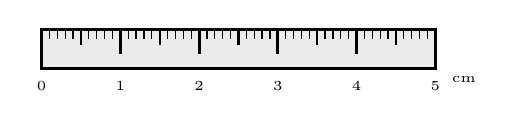
\begin{tikzpicture}[x=1cm, y=1cm, every node/.style={font=\scriptsize, text=black}]
      \draw[black, line width=1.1pt, fill=panelgray] (0,0) rectangle (5.0, 0.50);
      \foreach \m in {0,...,50}{
        \pgfmathsetmacro{\xval}{\m*0.1}
        \draw[black, line width=0.45pt] (\xval, 0.50) -- (\xval, 0.38);
      }
      \foreach \h in {0,0.5,...,5.0}{
        \draw[black, line width=0.8pt] (\h, 0.50) -- (\h, 0.30);
      }
      \foreach \c in {0,1,2,3,4,5}{
        \draw[black, line width=1.1pt] (\c, 0.50) -- (\c, 0.19);
        \node[below=1pt, font=\tiny] at (\c, 0.0) {\en{\c}};
      }
      \node[right=2pt, font=\tiny] at (5.02, -0.14) {\en{cm}};
    \end{tikzpicture}
  \end{tcolorbox}
\end{minipage}

\vspace{3pt}

% --- ផ្នែកទី ១៖ បន្ទះកាត់គ្រោងដំបូល 3-របារ (6, 5, 3 cm) + បន្ថែម 4-របារ (4 cm) + បន្ទះតេស្តមិនកើត (2, 2.5, 6 cm) ---
\textbf{១. សកម្មភាព \en{1} ៖ បន្ទះក្រដាសកាត់តាមស្នាមចុច \scissors{} (ខ្នាតពិត \en{x=1cm, y=1cm} \en{--} ចម្ងាយរវាងចំណុចកណ្ដាលរន្ធ \en{o} ទាំងពីរ)}

\vspace{1.5pt}
\begin{center}
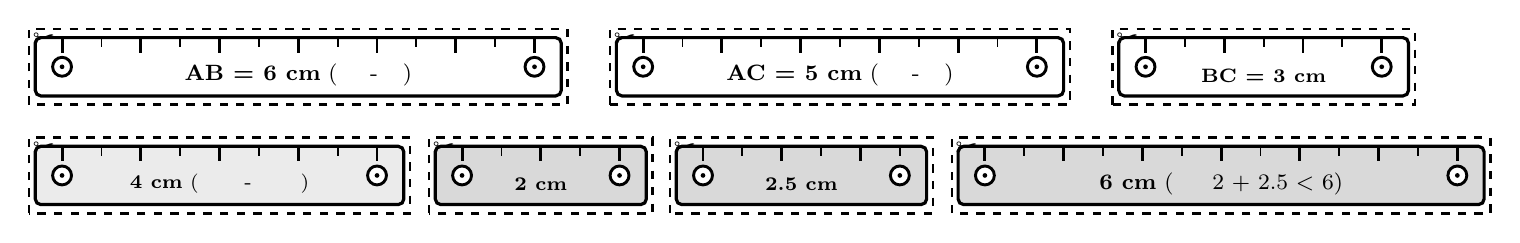
\begin{tikzpicture}[x=1cm, y=1cm, every node/.style={font=\scriptsize, text=black}]
  % === ជួរទី ១៖ ឈុតគ្រោងដំបូល ៣ របាររឹងថេរ (AB=6cm, AC=5cm, BC=3cm) ===
  % 6 cm
  \begin{scope}[shift={(0.42, 1.38)}]
    \draw[black, dashed, line width=0.95pt] (-0.42, -0.48) rectangle (6.42, 0.48);
    \node[anchor=north west, inner sep=1pt, font=\footnotesize] at (-0.41, 0.47) {\scissors};
    \draw[black, line width=1.15pt, rounded corners=2pt, fill=white] (-0.34, -0.37) rectangle (6.34, 0.37);
    \foreach \h in {0,0.5,...,6.0}{\draw[black, line width=0.65pt] (\h, 0.37) -- (\h, 0.25);}
    \foreach \k in {0,...,6}{\draw[black, line width=1.05pt] (\k, 0.37) -- (\k, 0.18);}
    \draw[black, line width=1.05pt, fill=white] (0,0) circle (0.12); \fill[black] (0,0) circle (0.03);
    \draw[black, line width=1.05pt, fill=white] (6,0) circle (0.12); \fill[black] (6,0) circle (0.03);
    \node[font=\footnotesize] at (3.0, -0.11) {\textbf{\en{AB = 6 cm}} (ឈុត ៣-របារ)};
  \end{scope}
  % 5 cm
  \begin{scope}[shift={(7.80, 1.38)}]
    \draw[black, dashed, line width=0.95pt] (-0.42, -0.48) rectangle (5.42, 0.48);
    \node[anchor=north west, inner sep=1pt, font=\footnotesize] at (-0.41, 0.47) {\scissors};
    \draw[black, line width=1.15pt, rounded corners=2pt, fill=white] (-0.34, -0.37) rectangle (5.34, 0.37);
    \foreach \h in {0,0.5,...,5.0}{\draw[black, line width=0.65pt] (\h, 0.37) -- (\h, 0.25);}
    \foreach \k in {0,...,5}{\draw[black, line width=1.05pt] (\k, 0.37) -- (\k, 0.18);}
    \draw[black, line width=1.05pt, fill=white] (0,0) circle (0.12); \fill[black] (0,0) circle (0.03);
    \draw[black, line width=1.05pt, fill=white] (5,0) circle (0.12); \fill[black] (5,0) circle (0.03);
    \node[font=\footnotesize] at (2.5, -0.11) {\textbf{\en{AC = 5 cm}} (ឈុត ៣-របារ)};
  \end{scope}
  % 3 cm
  \begin{scope}[shift={(14.18, 1.38)}]
    \draw[black, dashed, line width=0.95pt] (-0.42, -0.48) rectangle (3.42, 0.48);
    \node[anchor=north west, inner sep=1pt, font=\footnotesize] at (-0.41, 0.47) {\scissors};
    \draw[black, line width=1.15pt, rounded corners=2pt, fill=white] (-0.34, -0.37) rectangle (3.34, 0.37);
    \foreach \h in {0,0.5,...,3.0}{\draw[black, line width=0.65pt] (\h, 0.37) -- (\h, 0.25);}
    \foreach \k in {0,...,3}{\draw[black, line width=1.05pt] (\k, 0.37) -- (\k, 0.18);}
    \draw[black, line width=1.05pt, fill=white] (0,0) circle (0.12); \fill[black] (0,0) circle (0.03);
    \draw[black, line width=1.05pt, fill=white] (3,0) circle (0.12); \fill[black] (3,0) circle (0.03);
    \node[font=\scriptsize] at (1.5, -0.11) {\textbf{\en{BC = 3 cm}}};
  \end{scope}

  % === ជួរទី ២៖ បន្ថែម 4 cm (ស៊ុម ៤-របាររង្គើ) + បន្ទះតេស្តមិនកើត (2 cm, 2.5 cm, 6 cm) ===
  % 4 cm
  \begin{scope}[shift={(0.42, 0.0)}]
    \draw[black, dashed, line width=0.95pt] (-0.42, -0.48) rectangle (4.42, 0.48);
    \node[anchor=north west, inner sep=1pt, font=\footnotesize] at (-0.41, 0.47) {\scissors};
    \draw[black, line width=1.15pt, rounded corners=2pt, fill=panelgray] (-0.34, -0.37) rectangle (4.34, 0.37);
    \foreach \h in {0,0.5,...,4.0}{\draw[black, line width=0.65pt] (\h, 0.37) -- (\h, 0.25);}
    \foreach \k in {0,...,4}{\draw[black, line width=1.05pt] (\k, 0.37) -- (\k, 0.18);}
    \draw[black, line width=1.05pt, fill=white] (0,0) circle (0.12); \fill[black] (0,0) circle (0.03);
    \draw[black, line width=1.05pt, fill=white] (4,0) circle (0.12); \fill[black] (4,0) circle (0.03);
    \node[font=\scriptsize] at (2.0, -0.11) {\textbf{\en{4 cm}} (បន្ថែម ៤-របារទ្រេត)};
  \end{scope}
  % 2 cm
  \begin{scope}[shift={(5.50, 0.0)}]
    \draw[black, dashed, line width=0.95pt] (-0.42, -0.48) rectangle (2.42, 0.48);
    \node[anchor=north west, inner sep=1pt, font=\footnotesize] at (-0.41, 0.47) {\scissors};
    \draw[black, line width=1.15pt, rounded corners=2pt, fill=headgray] (-0.34, -0.37) rectangle (2.34, 0.37);
    \foreach \h in {0,0.5,...,2.0}{\draw[black, line width=0.65pt] (\h, 0.37) -- (\h, 0.25);}
    \foreach \k in {0,1,2}{\draw[black, line width=1.05pt] (\k, 0.37) -- (\k, 0.18);}
    \draw[black, line width=1.05pt, fill=white] (0,0) circle (0.12); \fill[black] (0,0) circle (0.03);
    \draw[black, line width=1.05pt, fill=white] (2,0) circle (0.12); \fill[black] (2,0) circle (0.03);
    \node[font=\scriptsize] at (1.0, -0.11) {\textbf{\en{2 cm}}};
  \end{scope}
  % 2.5 cm
  \begin{scope}[shift={(8.56, 0.0)}]
    \draw[black, dashed, line width=0.95pt] (-0.42, -0.48) rectangle (2.92, 0.48);
    \node[anchor=north west, inner sep=1pt, font=\footnotesize] at (-0.41, 0.47) {\scissors};
    \draw[black, line width=1.15pt, rounded corners=2pt, fill=headgray] (-0.34, -0.37) rectangle (2.84, 0.37);
    \foreach \h in {0,0.5,...,2.5}{\draw[black, line width=0.65pt] (\h, 0.37) -- (\h, 0.25);}
    \foreach \k in {0,1,2}{\draw[black, line width=1.05pt] (\k, 0.37) -- (\k, 0.18);}
    \draw[black, line width=1.05pt, fill=white] (0,0) circle (0.12); \fill[black] (0,0) circle (0.03);
    \draw[black, line width=1.05pt, fill=white] (2.5,0) circle (0.12); \fill[black] (2.5,0) circle (0.03);
    \node[font=\scriptsize] at (1.25, -0.11) {\textbf{\en{2.5 cm}}};
  \end{scope}
  % 6 cm (for impossible check 2, 2.5, 6)
  \begin{scope}[shift={(12.14, 0.0)}]
    \draw[black, dashed, line width=0.95pt] (-0.42, -0.48) rectangle (6.42, 0.48);
    \node[anchor=north west, inner sep=1pt, font=\footnotesize] at (-0.41, 0.47) {\scissors};
    \draw[black, line width=1.15pt, rounded corners=2pt, fill=headgray] (-0.34, -0.37) rectangle (6.34, 0.37);
    \foreach \h in {0,0.5,...,6.0}{\draw[black, line width=0.65pt] (\h, 0.37) -- (\h, 0.25);}
    \foreach \k in {0,...,6}{\draw[black, line width=1.05pt] (\k, 0.37) -- (\k, 0.18);}
    \draw[black, line width=1.05pt, fill=white] (0,0) circle (0.12); \fill[black] (0,0) circle (0.03);
    \draw[black, line width=1.05pt, fill=white] (6,0) circle (0.12); \fill[black] (6,0) circle (0.03);
    \node[font=\footnotesize] at (3.0, -0.11) {\textbf{\en{6 cm}} (តេស្ត \en{2 + 2.5 < 6})};
  \end{scope}
\end{tikzpicture}
\end{center}

\vspace{2pt}

% --- ផ្នែកទី ២៖ ផ្ទាំងសង់ដោយដែកឈាន 1:1 (AB=6, r1=5, r2=3) + តេស្តមិនកើត (2, 2.5, 6 cm) ---
\textbf{២. ផ្ទាំងសង់ដោយដែកឈាន \en{1:1} និងតេស្តលក្ខខណ្ឌមិនអាចកើត (ខ្នាតពិត \en{x=1cm, y=1cm})}

\vspace{2pt}
\begin{center}
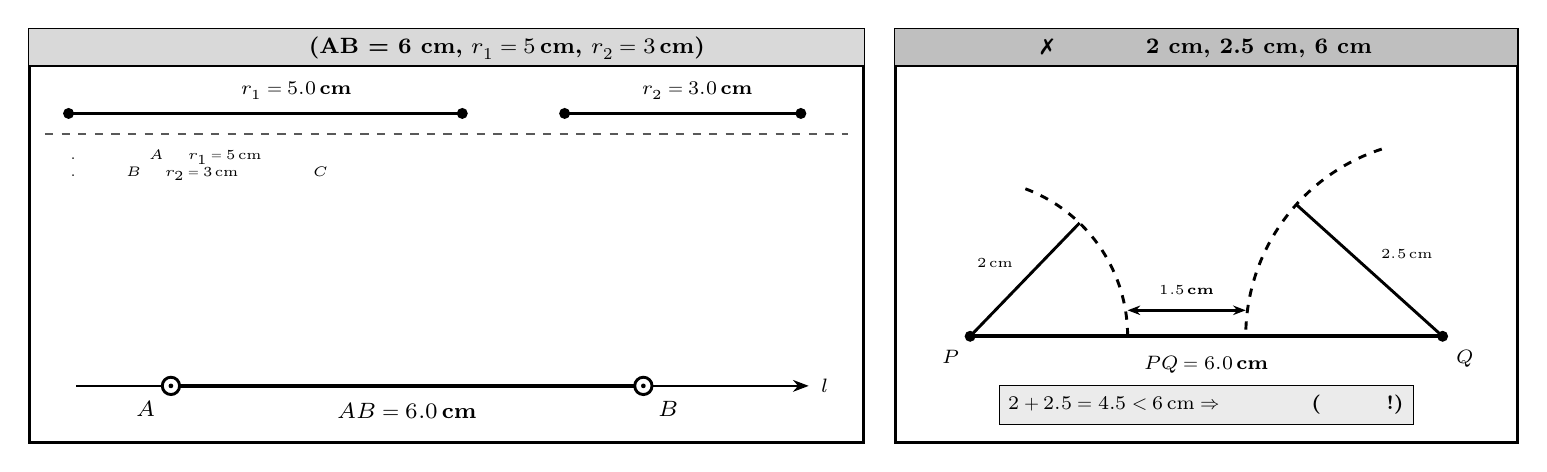
\begin{tikzpicture}[x=1cm, y=1cm, every node/.style={font=\scriptsize, text=black}]
  % === ខាងឆ្វេង៖ ផ្ទាំងសង់ដែកឈាន AB=6cm + កាំ r1=5cm, r2=3cm (10.6 cm wide x 5.25 cm high) ===
  \begin{scope}[shift={(0,0)}]
    \draw[black, line width=1.1pt] (0, 0) rectangle (10.6, 5.25);
    \fill[headgray] (0, 4.78) rectangle (10.6, 5.25);
    \draw[black, line width=0.9pt] (0, 4.78) -- (10.6, 4.78);
    \node[font=\footnotesize] at (5.30, 5.01) {\textbf{ផ្ទាំងសង់ដោយដែកឈាន (\en{AB = 6 cm}, $r_1=5\unit{cm}$, $r_2=3\unit{cm}$)}};

    % ខ្នាតកាំ r1 = 5.0 cm និង r2 = 3.0 cm ពិត 1:1 សម្រាប់បើកជើងដែកឈាន
    \draw[black, line width=1.2pt] (0.50, 4.18) -- (5.50, 4.18);
    \fill[black] (0.50, 4.18) circle (0.07) (5.50, 4.18) circle (0.07);
    \node[above=1pt, font=\scriptsize] at (3.00, 4.20) {បើកដែកឈាន៖ \textbf{$r_1 = 5.0\unit{cm}$}};

    \draw[black, line width=1.2pt] (6.80, 4.18) -- (9.80, 4.18);
    \fill[black] (6.80, 4.18) circle (0.07) (9.80, 4.18) circle (0.07);
    \node[above=1pt, font=\scriptsize] at (8.30, 4.20) {កាំ៖ \textbf{$r_2 = 3.0\unit{cm}$}};

    \draw[darkline, dashed, line width=0.7pt] (0.2, 3.92) -- (10.4, 3.92);

    % បន្ទាត់ l និងអង្កត់ AB = 6.0 cm ពិត (x=1.8 ដល់ x=7.8, y=0.75)
    \coordinate (A) at (1.80, 0.72);
    \coordinate (B) at (7.80, 0.72);
    \draw[black, line width=0.85pt, -{Stealth[length=2mm]}] (0.60, 0.72) -- (9.90, 0.72) node[right=1pt, font=\scriptsize] {$l$};
    \draw[black, line width=1.4pt] (A) -- (B) node[midway, below=2pt, font=\footnotesize] {\textbf{$AB = 6.0\unit{cm}$}};
    \draw[black, line width=1.05pt, fill=white] (A) circle (0.11); \fill[black] (A) circle (0.03);
    \draw[black, line width=1.05pt, fill=white] (B) circle (0.11); \fill[black] (B) circle (0.03);
    \node[below left=2pt, font=\footnotesize] at (A) {$A$};
    \node[below right=2pt, font=\footnotesize] at (B) {$B$};

    \node[anchor=north west, font=\tiny, align=left] at (0.35, 3.84) {១. ដាក់ដែកឈានត្រង់ $A$ កាំ $r_1=5\unit{cm}$ គូសធ្នូ\\២. ដាក់ត្រង់ $B$ កាំ $r_2=3\unit{cm}$ គូសធ្នូកាត់ត្រង់ $C$};
  \end{scope}

  % === ខាងស្ដាំ៖ ផ្ទាំងមើលជាមុន 2 + 2.5 < 6 cm ពិត 1:1 (7.9 cm wide x 5.25 cm high) ===
  \begin{scope}[shift={(11.0, 0)}]
    \draw[black, line width=1.1pt] (0, 0) rectangle (7.90, 5.25);
    \fill[midgray] (0, 4.78) rectangle (7.90, 5.25);
    \draw[black, line width=0.9pt] (0, 4.78) -- (7.90, 4.78);
    \node[font=\footnotesize] at (3.95, 5.01) {\textbf{\ding{55}\ តេស្តមិនកើត៖ \en{2 cm, 2.5 cm, 6 cm}}};

    % អង្កត់គោល PQ = 6.0 cm (x=0.95 ដល់ x=6.95, y=1.35)
    \coordinate (P) at (0.95, 1.35);
    \coordinate (Q) at (6.95, 1.35);
    \draw[black, line width=1.35pt] (P) -- (Q) node[midway, below=3pt, font=\scriptsize] {\textbf{$PQ = 6.0\unit{cm}$}};
    \fill[black] (P) circle (0.07) node[below left=1.5pt] {$P$};
    \fill[black] (Q) circle (0.07) node[below right=1.5pt] {$Q$};

    % ធ្នូកាំ 2.0 cm ពី P និង 2.5 cm ពី Q (គម្លាត 1.5 cm, មិនធ្លាក់ក្រោម PQ ទេ!)
    \draw[black, line width=1.05pt, dashed] ($(P)+(0:2.0)$) arc (0:72:2.0);
    \draw[black, line width=1.05pt] (P) -- ($(P)+(46:2.0)$) node[midway, above left=0.5pt, font=\tiny] {$2\unit{cm}$};
    \draw[black, line width=1.05pt, dashed] ($(Q)+(108:2.5)$) arc (108:180:2.5);
    \draw[black, line width=1.05pt] (Q) -- ($(Q)+(138:2.5)$) node[midway, above right=0.5pt, font=\tiny] {$2.5\unit{cm}$};

    % ចន្លោះប្រហោង 1.5 cm (ពី x=2.95 ដល់ x=4.45)
    \draw[black, line width=0.95pt, {Stealth[length=1.6mm]}-{Stealth[length=1.6mm]}] (2.95, 1.68) -- (4.45, 1.68);
    \node[above=1pt, font=\tiny, align=center] at (3.70, 1.72) {\textbf{ប្រហោង}\\\textbf{$1.5\unit{cm}$}};

    \node[draw=black, fill=panelgray, inner sep=3.5pt, align=center, font=\scriptsize] at (3.95, 0.48) {$2 + 2.5 = 4.5 < 6\unit{cm} \Rightarrow$ \textbf{ធ្នូមិនប៉ះគ្នា (គ្មានត្រីកោណ!)}};
  \end{scope}
\end{tikzpicture}
\end{center}

\vspace{2pt}

% --- ផ្នែកទី ៣៖ សកម្មភាព 2 POE បដិឧទាហរណ៍ AAA (4 cm vs 6 cm មុំ 60°-60°-60°, x=1cm, y=1cm) ---
\textbf{៣. សកម្មភាព \en{2} \en{POE} \en{:} បដិឧទាហរណ៍អន្ទាក់ ម.ម.ម (\en{AAA} \en{--} មុំ $60^\circ\text{-}60^\circ\text{-}60^\circ$, ខ្នាតពិត \en{x=1cm, y=1cm})}

\vspace{2pt}
\noindent
\begin{minipage}[c]{12.15cm}
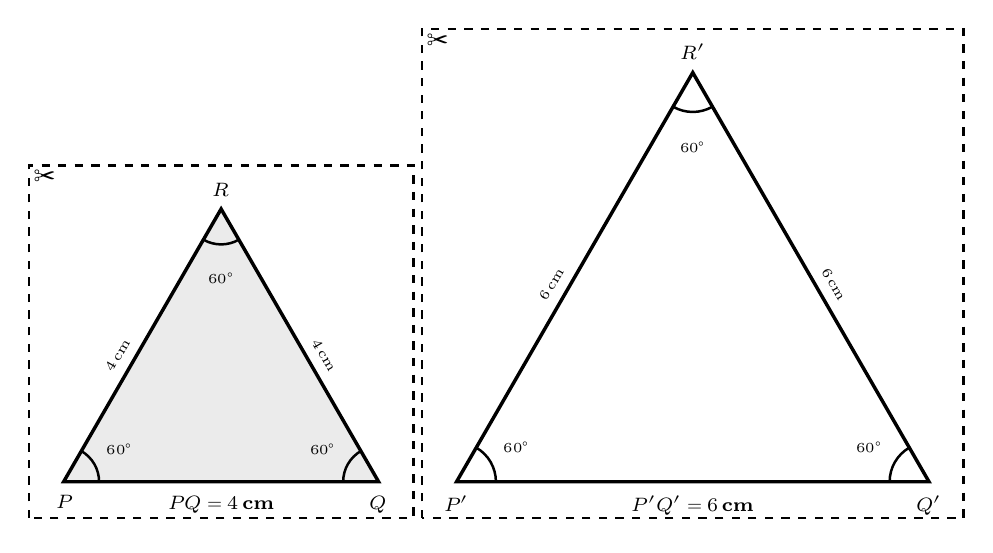
\begin{tikzpicture}[x=1cm, y=1cm, every node/.style={font=\scriptsize, text=black}]
  % === ត្រីកោណសម័ង្ស PQR ជ្រុងពិត 4.0 cm ===
  \begin{scope}[shift={(0.46, 0.48)}]
    \draw[black, dashed, line width=0.95pt] (-0.44, -0.46) rectangle (4.44, 4.02);
    \node[anchor=north west, inner sep=1pt, font=\footnotesize] at (-0.42, 4.00) {\scissors};
    \coordinate (P) at (0,0);
    \coordinate (Q) at (4.0,0);
    \coordinate (R) at (2.0, 3.4641);
    \fill[panelgray] (P) -- (Q) -- (R) -- cycle;
    \draw[black, line width=1.25pt] (P) -- (Q) -- (R) -- cycle;
    \pic[draw=black, line width=0.9pt, angle radius=4.5mm]{angle=Q--P--R};
    \pic[draw=black, line width=0.9pt, angle radius=4.5mm]{angle=R--Q--P};
    \pic[draw=black, line width=0.9pt, angle radius=4.5mm]{angle=P--R--Q};
    \node[font=\tiny] at ($(P)+(30:0.82)$) {$60^\circ$};
    \node[font=\tiny] at ($(Q)+(150:0.82)$) {$60^\circ$};
    \node[font=\tiny] at ($(R)+(-90:0.88)$) {$60^\circ$};
    \node[below=1.5pt, font=\scriptsize] at (2.0, 0) {\textbf{$PQ = 4\unit{cm}$}};
    \node[above left=0.5pt, rotate=60, font=\tiny] at ($(P)!0.52!(R)$) {$4\unit{cm}$};
    \node[above right=0.5pt, rotate=-60, font=\tiny] at ($(Q)!0.52!(R)$) {$4\unit{cm}$};
    \node[below=1.5pt] at (P) {$P$};
    \node[below=1.5pt] at (Q) {$Q$};
    \node[above=1pt] at (R) {$R$};
  \end{scope}

  % === ត្រីកោណសម័ង្ស P'Q'R' ជ្រុងពិត 6.0 cm ===
  \begin{scope}[shift={(5.45, 0.48)}]
    \draw[black, dashed, line width=0.95pt] (-0.44, -0.46) rectangle (6.44, 5.75);
    \node[anchor=north west, inner sep=1pt, font=\footnotesize] at (-0.42, 5.73) {\scissors};
    \coordinate (Pp) at (0,0);
    \coordinate (Qp) at (6.0,0);
    \coordinate (Rp) at (3.0, 5.1962);
    \fill[white] (Pp) -- (Qp) -- (Rp) -- cycle;
    \draw[black, line width=1.25pt] (Pp) -- (Qp) -- (Rp) -- cycle;
    \pic[draw=black, line width=0.9pt, angle radius=5.0mm]{angle=Qp--Pp--Rp};
    \pic[draw=black, line width=0.9pt, angle radius=5.0mm]{angle=Rp--Qp--Pp};
    \pic[draw=black, line width=0.9pt, angle radius=5.0mm]{angle=Pp--Rp--Qp};
    \node[font=\tiny] at ($(Pp)+(30:0.88)$) {$60^\circ$};
    \node[font=\tiny] at ($(Qp)+(150:0.88)$) {$60^\circ$};
    \node[font=\tiny] at ($(Rp)+(-90:0.95)$) {$60^\circ$};
    \node[below=1.5pt, font=\scriptsize] at (3.0, 0) {\textbf{$P'Q' = 6\unit{cm}$}};
    \node[above left=0.5pt, rotate=60, font=\tiny] at ($(Pp)!0.52!(Rp)$) {$6\unit{cm}$};
    \node[above right=0.5pt, rotate=-60, font=\tiny] at ($(Qp)!0.52!(Rp)$) {$6\unit{cm}$};
    \node[below=1.5pt] at (Pp) {$P'$};
    \node[below=1.5pt] at (Qp) {$Q'$};
    \node[above=1pt] at (Rp) {$R'$};
  \end{scope}
\end{tikzpicture}
\end{minipage}%
\hfill
\begin{minipage}[c]{6.55cm}
  \begin{tcolorbox}[
    enhanced, sharp corners, colback=white, colframe=black,
    boxrule=1.05pt, boxsep=1pt, top=4pt, bottom=4pt, left=5pt, right=5pt,
    title={\textbf{កំណត់ត្រា \en{POE} (សកម្មភាព ១ \& ២)}},
    colbacktitle=headgray, coltitle=black, fonttitle=\fontsize{8.5pt}{11.5pt}\selectfont
  ]
    \raggedright\fontsize{8.1pt}{11.8pt}\selectfont
    \textbf{សកម្មភាព ១ (ស៊ុមដំបូល)៖}\\
    \chkbox\ ៣ របារ ($6,5,3\unit{cm}$): \underline{\hspace{2.1cm}}\\
    \chkbox\ ៤ របារ ($6,5,4,3\unit{cm}$): \underline{\hspace{1.9cm}}\\[4pt]
    \textbf{\en{P} \en{--} ទស្សន៍ទាយ (\en{AAA} $60^\circ$):}\\
    មុំទាំង ៣ ស្មើ $60^\circ$ តើត្រីកោណប៉ុនគ្នាទេ?\\
    \chkbox\ ប៉ុនគ្នា \hspace{0.3cm} \chkbox\ មិនប្រាកដ\\[4pt]
    \textbf{\en{O} \en{--} សង្កេត (កាត់ផ្ទៀងត្រួត)៖}\\
    ដាក់ $\tri{PQR}$ ($4\unit{cm}$) លើ $\tri{P'Q'R'}$ ($6\unit{cm}$)៖\\
    \chkbox\ ត្រួតបេះបិទ \hspace{0.15cm} \chkbox\ តូចជាង ($\ncg$)\\[4pt]
    \textbf{\en{E} \en{--} ពន្យល់៖} ហេតុអ្វី \textbf{ម.ម.ម (\en{AAA})} មិនគ្រប់គ្រាន់ តែ \textbf{ជ.ជ.ជ (\en{SSS})} គ្រប់គ្រាន់?\\[4pt]
    \rule{\linewidth}{0.55pt}\\[10pt]
    \rule{\linewidth}{0.55pt}\\[10pt]
    \rule{\linewidth}{0.55pt}
  \end{tcolorbox}
\end{minipage}

\clearpage

% ============================================================================
% ទំព័រទី ២៖ E4 Elaborate — កាតសកម្មភាព "ស្ពានតភ្ជាប់អង្កត់ & គំនូស ៣ កម្រិត" (២ ប័ណ្ណ)
% ============================================================================
\pagebanner{សម្ភារៈទី ២៖ កាតស៊ើបអង្កេត «ស្ពានតភ្ជាប់អង្កត់ \enbf{\&} គំនូស \enbf{|, ||, |||}»}{ទំព័រ ២/៦ \en{-- E4 Elaborate} (កាត់ ២ ប័ណ្ណ \scissors)}

\newcommand{\eFourCard}[1]{%
\begin{tcolorbox}[
  enhanced, sharp corners, colback=white, colframe=white,
  borderline={1.0pt}{0pt}{black, dashed},
  boxsep=1pt, top=4pt, bottom=4pt, left=5pt, right=5pt
]
  \begin{tcolorbox}[
    enhanced, sharp corners, colback=headgray, colframe=black,
    boxrule=0.8pt, boxsep=1pt, top=2.5pt, bottom=2.5pt, left=5pt, right=5pt, after skip=5pt
  ]
    \fontsize{8.5pt}{11.5pt}\selectfont
    \textbf{\scissors\ កាតសកម្មភាព \en{E4} (#1) \en{--} ស្ពានតភ្ជាប់អង្កត់ \en{JG} និងគំនូស \tickone, \ticktwo, \tickthree} \hfill ក្រុម៖ $\underline{\hspace{2.8cm}}$
  \end{tcolorbox}

  \noindent
  \begin{minipage}[t]{7.4cm}
    \vspace{0pt}
    \fontsize{8.3pt}{11.8pt}\selectfont
    \textbf{លំហាត់គំរូ (សៀវភៅទំព័រ ១៥២)៖} ក្នុងរូបខាងក្រោម គេឱ្យ $EF = HK$, $FJ = GK$ និង $EG = HJ$ ($F\text{-}J\text{-}G\text{-}K$ ត្រង់ជួរដេក) ។ ចូរបង្ហាញថា $\tri{EFG} \cg \tri{HKJ}$ ។
    \begin{center}
    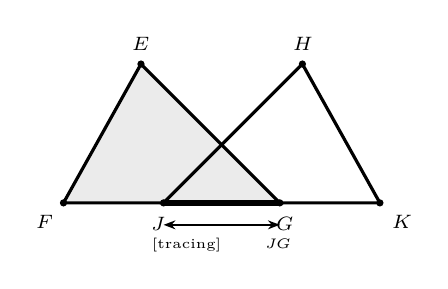
\begin{tikzpicture}[scale=0.82, every node/.style={font=\scriptsize, text=black}]
      % F-J-G-K collinear horizontal (Book p. 152)
      \coordinate (F) at (0,0);
      \coordinate (J) at (1.55,0);
      \coordinate (G) at (3.35,0);
      \coordinate (K) at (4.90,0);
      \coordinate (E) at (1.20, 2.15);
      \coordinate (H) at (3.70, 2.15);
      \fill[panelgray] (E) -- (F) -- (G) -- cycle;
      \draw[black, line width=1.15pt] (E) -- (F) -- (G) -- cycle;
      \draw[black, line width=1.15pt] (H) -- (J) -- (K) -- cycle;
      % Finger-trace highlight on shared bridge JG
      \draw[black, line width=2.4pt] (J) -- (G);
      \draw[black, line width=0.85pt, {Stealth[length=1.5mm]}-{Stealth[length=1.5mm]}] (1.55, -0.34) -- (3.35, -0.34);
      \node[below=1pt, font=\tiny] at (2.45, -0.35) {\en{[tracing]} ស្ពានរួម $JG$};
      \fill[black] (F) circle (1.6pt) node[below left=1pt] {$F$};
      \fill[black] (J) circle (1.6pt) node[below=1.5pt, xshift=-2pt] {$J$};
      \fill[black] (G) circle (1.6pt) node[below=1.5pt, xshift=2pt] {$G$};
      \fill[black] (K) circle (1.6pt) node[below right=1pt] {$K$};
      \fill[black] (E) circle (1.6pt) node[above=1.5pt] {$E$};
      \fill[black] (H) circle (1.6pt) node[above=1.5pt] {$H$};
    \end{tikzpicture}
    \end{center}
    \begin{tcolorbox}[enhanced, sharp corners, colback=panelgray, colframe=black, boxrule=0.7pt, boxsep=1pt, top=2.5pt, bottom=2.5pt, left=4pt, right=4pt]
      \fontsize{7.7pt}{11.0pt}\selectfont
      \textbf{ពិនិត្យក្រោយ (\en{EIA} ៣០ វិនាទី)៖} បើរំកិល $\tri{HKJ}$ តាមបន្ទាត់ $FK$ ដោយរក្សា $FJ=GK$ តើ $JG, FG$ ប្រែប្រួលទេ? ចុះ $FG=JK$?\\
      \chkbox\ $FG=JK$ នៅពិតជានិច្ច \hspace{0.1cm} \chkbox\ ប្រែប្រួល
    \end{tcolorbox}
  \end{minipage}\hfill
  \begin{minipage}[t]{10.4cm}
    \vspace{0pt}
    \begin{tcolorbox}[enhanced, sharp corners, colback=panelgray, colframe=black, boxrule=0.8pt, boxsep=1pt, top=3.5pt, bottom=3.5pt, left=5pt, right=5pt]
      \raggedright\fontsize{8.1pt}{12.3pt}\selectfont
      \textbf{ជំហាន ១ [ចង្អុល \en{[tracing]} និងគូស \tickone, \ticktwo, \tickthree\ លើរូប]៖}\\
      \chkbox\ គូស \tickone\ លើ $EF = \underline{\hspace{0.9cm}}$ (\cnum{1}) \hspace{0.15cm}
      \chkbox\ គូស \ticktwo\ លើ $EG = \underline{\hspace{0.9cm}}$ (\cnum{1})\\
      \chkbox\ ចង្អុលម្រាមដៃ \en{[tracing]} តាមស្ពាន $JG$ រួចគូស \tickthree\ លើ $FG$ និង $JK$!\\[4pt]
      \textbf{ជំហាន ២ [ស្ពានតភ្ជាប់អង្កត់រួម \cnum{2}]៖}\\
      ដោយ $FJ = GK$ (\cnum{1} បម្រាប់) និង $JG$ ជាអង្កត់រួម៖\\
      $FG = FJ + \underline{\hspace{1.15cm}} = \underline{\hspace{1.15cm}} + GK = JK$ \hspace{0.15cm} (\cnum{2} $\underline{\hspace{1.8cm}}$)\\[4pt]
      \textbf{ជំហាន ៣ [ផ្ទៀង ជ.ជ.ជ \cnum{4} \& កំពូលឈមជ្រុងស្មើ \cnum{5}]៖}\\
      ក្នុង $\tri{EFG}$ និង $\tri{HKJ}$ មាន៖\\
      \en{1)} $EF = \underline{\hspace{1.0cm}}$ (\cnum{1}) \hspace{0.15cm}
      \en{2)} $EG = \underline{\hspace{1.0cm}}$ (\cnum{1}) \hspace{0.15cm}
      \en{3)} $FG = \underline{\hspace{1.0cm}}$ (\cnum{2})\\
      ដូចនេះ $\tri{EFG}\;\underline{\hspace{0.45cm}}\;\tri{HKJ}$ \hspace{0.15cm} (\cnum{4} $\underline{\hspace{1.7cm}}$)\\
      \textbf{វិបាក (\cnum{5})៖} $\ang{E}=\ang{\underline{\hspace{0.6cm}}}$ (ឈម $FG, JK$), $\ang{F}=\ang{\underline{\hspace{0.6cm}}}$, $\ang{G}=\ang{\underline{\hspace{0.6cm}}}$
    \end{tcolorbox}
    \vspace{3pt}
    {\fontsize{7.5pt}{10.5pt}\selectfont
    \textbf{ធនាគារអំណះអំណាង៖} \cnum{1} បម្រាប់ \en{|} \cnum{2} បូក/ដកអង្កត់រួម \en{|} \cnum{3} ជ្រុងរួម \en{|} \cnum{4} ជ.ជ.ជ \en{|} \cnum{5} ធាតុត្រូវគ្នា}
  \end{minipage}
\end{tcolorbox}%
}

\eFourCard{ប័ណ្ណទី ១}

\vspace{8pt}
\noindent\scissors\ \dotfill\ \textbf{កាត់តាមស្នាមចុចចែកជា ២ ប័ណ្ណ (\en{Cut Along Dashed Line})} \dotfill\ \scissors
\vspace{8pt}

\eFourCard{ប័ណ្ណទី ២}

\clearpage

% ============================================================================
% ទំព័រទី ៣៖ E5 Evaluate — សន្លឹកអធិការកិច្ចប្លង់ ៣ តួនាទី (២ ប័ណ្ណ)
% ============================================================================
\pagebanner{សម្ភារៈទី ៣៖ សន្លឹក «ក្រុមអធិការកិច្ចប្លង់ ៣ តួនាទី» \enbf{--} ប្រតិបត្តិ \enbf{E5 \& E1}}{ទំព័រ ៣/៦ \en{-- E5 Evaluate} (កាត់ ២ សន្លឹក \scissors)}

\newcommand{\eFiveSheet}[1]{%
\begin{tcolorbox}[
  enhanced, sharp corners, colback=white, colframe=white,
  borderline={1.0pt}{0pt}{black, dashed},
  boxsep=1pt, top=3.5pt, bottom=3.5pt, left=4.5pt, right=4.5pt
]
  \begin{tcolorbox}[
    enhanced, sharp corners, colback=headgray, colframe=black,
    boxrule=0.8pt, boxsep=1pt, top=2pt, bottom=2pt, left=5pt, right=5pt, after skip=4pt
  ]
    \fontsize{8.1pt}{11pt}\selectfont
    \textbf{\scissors\ សន្លឹកអធិការកិច្ចប្លង់ (#1) \en{--} ក្រុមជាងសំណង់ដំបូល៖} $\underline{\hspace{2.2cm}}$ \hfill \textbf{ប្រតិបត្តិ (ទំព័រ ១៥៣)៖} $RZ=VW,\; TZ=SW,\; RS=TV$ $\Rightarrow$ ប្រៀបធៀប $\tri{RZT}, \tri{VWS}$
  \end{tcolorbox}

  \renewcommand{\arraystretch}{1.06}
  \begin{tabular}{|L{5.30cm}|L{6.25cm}|L{5.55cm}|}
    \hline
    \cellcolor{panelgray}\centering\arraybackslash\fontsize{7.8pt}{10.5pt}\selectfont\textbf{តួនាទី ១៖ អ្នកគូសសញ្ញា \tickone, \ticktwo, \tickthree}\newline {\fontsize{7.2pt}{9.5pt}\selectfont \textbf{\en{Pause-Ask!}} \en{--} និយាយមាត់មុនគូស} &
    \cellcolor{panelgray}\centering\arraybackslash\fontsize{7.8pt}{10.5pt}\selectfont\textbf{តួនាទី ២៖ អ្នកតភ្ជាប់អង្កត់ \& \cnum{1}--\cnum{4}}\newline {\fontsize{7.2pt}{9.5pt}\selectfont សរសេរស្ពានឈរ \& បំពេញហេតុផល} &
    \cellcolor{panelgray}\centering\arraybackslash\fontsize{7.8pt}{10.5pt}\selectfont\textbf{តួនាទី ៣៖ អ្នកផ្ទៀងកំពូល \& វិបាក \cnum{5}}\newline {\fontsize{7.2pt}{9.5pt}\selectfont \textbf{\en{Pause-Review!}} \en{+} បិទបេសកកម្ម \en{E1}} \\ \hline
    {\fontsize{7.4pt}{10pt}\selectfont\textbf{រូបប្រតិបត្តិ (ទំព័រ ១៥៣)៖}\par}
    \vspace{1pt}
    {\centering
    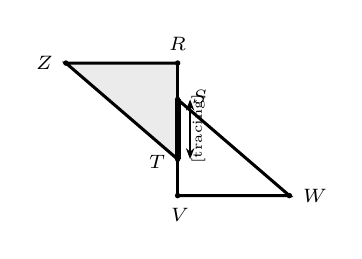
\begin{tikzpicture}[scale=0.66, every node/.style={font=\scriptsize, text=black}]
      % Exact vertical collinear R-S-T-V (Book p. 153)
      \coordinate (R) at (0, 2.55);
      \coordinate (S) at (0, 1.85);
      \coordinate (T) at (0, 0.70);
      \coordinate (V) at (0, 0.00);
      \coordinate (Z) at (-2.15, 2.55);
      \coordinate (W) at (2.15, 0.00);
      \fill[panelgray] (R) -- (Z) -- (T) -- cycle;
      \draw[black, line width=1.1pt] (R) -- (V);
      \draw[black, line width=1.1pt] (R) -- (Z) -- (T);
      \draw[black, line width=1.1pt] (V) -- (W) -- (S);
      % [tracing] cue on vertical shared bridge ST (vertical text so zero touch on SW)
      \draw[black, line width=2.2pt] (S) -- (T);
      \draw[black, line width=0.8pt, {Stealth[length=1.4mm]}-{Stealth[length=1.4mm]}] (0.24, 1.85) -- (0.24, 0.70);
      \node[rotate=90, font=\tiny, inner sep=0.5pt] at (0.40, 1.28) {\en{[tracing]}};
      \fill[black] (R) circle (1.5pt) node[above=1pt] {$R$};
      \fill[black] (S) circle (1.5pt) node[right=2pt, yshift=1pt] {$S$};
      \fill[black] (T) circle (1.5pt) node[left=2pt, yshift=-1pt] {$T$};
      \fill[black] (V) circle (1.5pt) node[below=1pt] {$V$};
      \fill[black] (Z) circle (1.5pt) node[left=1.5pt] {$Z$};
      \fill[black] (W) circle (1.5pt) node[right=1.5pt] {$W$};
    \end{tikzpicture}\par}
    \fontsize{7.4pt}{10.5pt}\selectfont
    \chkbox\ គូស \tickone\ ($RS=TV$), \ticktwo\ ($RZ=VW$), \tickthree\ ($TZ=SW$)\newline
    \chkbox\ \textbf{\en{Pause-Ask!}} «ហេតុអ្វី $RT=SV$? (ហាមគូសមុំមុនស្រាយ!)»
    &
    \fontsize{7.8pt}{11.8pt}\selectfont
    \textbf{ស្ពានឈរ (\cnum{2})៖}\newline
    $RT = RS + \underline{\hspace{0.7cm}} = \underline{\hspace{0.7cm}} + TV = SV$\par\vspace{3pt}
    ក្នុង $\tri{RZT}$ និង $\tri{VWS}$ មាន៖\par\vspace{2pt}
    \en{1)} $RZ = \underline{\hspace{0.95cm}}$ (\cnum{1} $\underline{\hspace{1.25cm}}$)\par\vspace{2.5pt}
    \en{2)} $TZ = \underline{\hspace{0.95cm}}$ (\cnum{1} $\underline{\hspace{1.25cm}}$)\par\vspace{2.5pt}
    \en{3)} $RT = \underline{\hspace{0.95cm}}$ (\cnum{2} $\underline{\hspace{1.25cm}}$)\par\vspace{3pt}
    ដូចនេះ $\tri{\underline{\hspace{0.85cm}}} \cg \tri{\underline{\hspace{0.85cm}}}$ (\cnum{4} $\underline{\hspace{0.95cm}}$)\par\vspace{3pt}
    {\fontsize{6.9pt}{9.5pt}\selectfont ធនាគារ៖ \cnum{1} បម្រាប់ \cnum{2} បូកអង្កត់រួម \cnum{3} ជ្រុងរួម \cnum{4} ជ.ជ.ជ}
    &
    \fontsize{7.7pt}{11.5pt}\selectfont
    \chkbox\ \textbf{\en{Pause-Review!}} ផ្ទៀងកំពូលឈមជ្រុង៖\newline
    $R\leftrightarrow\underline{\hspace{0.4cm}}$ (ឈម $TZ,SW$),\; $Z\leftrightarrow\underline{\hspace{0.4cm}}$,\; $T\leftrightarrow\underline{\hspace{0.4cm}}$\par\vspace{2pt}
    \chkbox\ ប្រើ $=$ (ប្រវែង/មុំ) ទល់ $\cg$ (ត្រីកោណ)\par\vspace{3pt}
    \textbf{វិបាក (\cnum{5})៖} $\ang{R}=\ang{\underline{\hspace{0.5cm}}}$, $\ang{Z}=\ang{\underline{\hspace{0.5cm}}}$, $\ang{T}=\ang{\underline{\hspace{0.5cm}}}$\par\vspace{3pt}
    \textbf{បិទ \en{E1} (ដំបូល $6\unit{m},5\unit{m},3\unit{m}$)៖} មិនវាស់មុំ ប៉ុនគ្នាដោយ \cnum{4} $\underline{\hspace{0.9cm}}$ $\Rightarrow$ មុំដំបូលស្មើដោយ \cnum{5}!
    \\[1pt] \hline
  \end{tabular}
\end{tcolorbox}%
}

\eFiveSheet{សន្លឹកទី ១}

\vspace{6pt}
\noindent\scissors\ \dotfill\ \textbf{កាត់តាមស្នាមចុចចែកជា ២ សន្លឹក (\en{Cut Along Dashed Line})} \dotfill\ \scissors
\vspace{6pt}

\eFiveSheet{សន្លឹកទី ២}

\clearpage

% ============================================================================
% ទំព័រទី ៤៖ ផ្ទាំងយោងប្រចាំថ្នាក់រៀន — ទ្រឹស្ដីបទ ជ.ជ.ជ កំពូលឈមជ្រុង & ធនាគារ ①–⑤
% ============================================================================
\begin{tcolorbox}[
  enhanced, sharp corners, colback=white, colframe=black,
  boxrule=1.5pt, borderline={0.6pt}{2.2pt}{black},
  boxsep=1pt, top=4.5pt, bottom=4.5pt, left=6pt, right=6pt
]
  \begin{center}
    {\muol\fontsize{11.5pt}{16pt}\selectfont ទ្រឹស្ដីបទ ជ\enbf{.}ជ\enbf{.}ជ \enbf{(SSS)} កំពូលឈមជ្រុងស្មើ និងធនាគារ \cnum{1}\en{--}\cnum{5}}\\[1pt]
    {\fontsize{8.8pt}{12.5pt}\selectfont ផ្ទាំងយោងប្រចាំថ្នាក់រៀន (ស-ខ្មៅ) \en{--} មេរៀនទី១២ (១.២.៣) ជ្រុងបីប៉ុនរៀងគ្នា}\\[2pt]
    \khmflourish
  \end{center}
  \vspace{1pt}

  % --- ផ្នែកទី ១៖ ទ្រឹស្ដីបទ + រូបបង្វិល ~135° & គោលការណ៍កំពូលឈមជ្រុង ---
  \noindent
  \begin{minipage}[c]{9.0cm}
    \begin{tcolorbox}[enhanced, sharp corners, colback=panelgray, colframe=black, boxrule=0.85pt, boxsep=1pt, top=3.5pt, bottom=3.5pt, left=5pt, right=5pt]
      \fontsize{8.1pt}{11.6pt}\selectfont
      \textbf{ទ្រឹស្ដីបទ (ជ.ជ.ជ)៖} ត្រីកោណពីរប៉ុនគ្នា កាលណាវាមានជ្រុងទាំងបីប៉ុនរៀងគ្នា។\\[3pt]
      \textbf{គោលការណ៍កំពូលឈមជ្រុងស្មើ (\en{Opposite-Angle Matching})៖} ទោះរូបបង្វិល\en{--}ឆ្លុះ $\approx 135^\circ$ ក៏កំពូលឈមជ្រុង \tickone\ ត្រូវនឹង \tickone, កំពូលឈមជ្រុង \ticktwo\ ត្រូវនឹង \ticktwo, កំពូលឈមជ្រុង \tickthree\ ត្រូវនឹង \tickthree!\\[2pt]
      \textbf{បែងចែកសញ្ញា៖} \textbf{$=$} សម្រាប់ប្រវែង/រង្វាស់មុំ \en{|} \textbf{$\cg$} សម្រាប់ត្រីកោណប៉ុនគ្នា។
    \end{tcolorbox}
  \end{minipage}\hfill
  \begin{minipage}[c]{8.8cm}
    \centering
    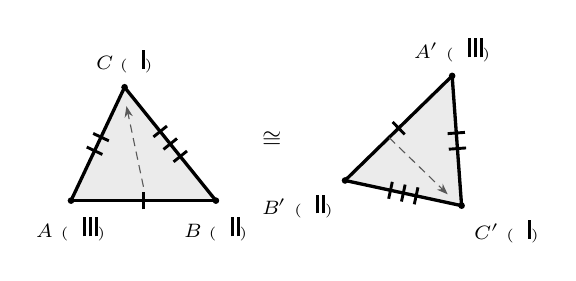
\begin{tikzpicture}[scale=0.80, every node/.style={font=\scriptsize, text=black}]
      % ត្រីកោណទី១
      \coordinate (A) at (0,0);
      \coordinate (B) at (2.30,0);
      \coordinate (C) at (0.85,1.80);
      \fill[panelgray] (A) -- (B) -- (C) -- cycle;
      \draw[black, line width=1.2pt, tk1] (A) -- (B);
      \draw[black, line width=1.2pt, tk2] (A) -- (C);
      \draw[black, line width=1.2pt, tk3] (B) -- (C);
      \fill[black] (A) circle (1.5pt) (B) circle (1.5pt) (C) circle (1.5pt);
      \node[below=2pt] at (A) {$A$ {\tiny(ឈម \tickthree)}};
      \node[below=2pt] at (B) {$B$ {\tiny(ឈម \ticktwo)}};
      \node[above=1.5pt] at (C) {$C$ {\tiny(ឈម \tickone)}};
      % ព្រួញភ្ជាប់ AB -> C
      \draw[darkline, densely dashed, -{Stealth[length=1.4mm]}] (1.15, 0.22) -- (0.88, 1.50);

      \node[font=\small] at (3.20, 0.98) {$\cg$};

      % ត្រីកោណទី២ (បង្វិល-ឆ្លុះ ~135 deg)
      \coordinate (Ap) at (6.05, 1.98);
      \coordinate (Bp) at (4.35, 0.32);
      \coordinate (Cp) at (6.20, -0.08);
      \fill[panelgray] (Ap) -- (Bp) -- (Cp) -- cycle;
      \draw[black, line width=1.2pt, tk1] (Ap) -- (Bp);
      \draw[black, line width=1.2pt, tk2] (Ap) -- (Cp);
      \draw[black, line width=1.2pt, tk3] (Bp) -- (Cp);
      \fill[black] (Ap) circle (1.5pt) (Bp) circle (1.5pt) (Cp) circle (1.5pt);
      \node[above=1.5pt] at (Ap) {$A'$ {\tiny(ឈម \tickthree)}};
      \node[below left=1pt] at (Bp) {$B'$ {\tiny(ឈម \ticktwo)}};
      \node[below right=1pt] at (Cp) {$C'$ {\tiny(ឈម \tickone)}};
      \draw[darkline, densely dashed, -{Stealth[length=1.4mm]}] (5.05, 1.00) -- (5.98, 0.10);
    \end{tikzpicture}
  \end{minipage}

  \vspace{4pt}

  % --- ផ្នែកទី ២៖ តារាង សម្មតិកម្ម-សន្និដ្ឋាន-វិបាក (កែកំហុសទំព័រ ១៥២ BC=B'C') ---
  \noindent
  \begin{minipage}[c]{9.2cm}
    \fontsize{8.0pt}{11.4pt}\selectfont
    \renewcommand{\arraystretch}{1.12}
    \begin{tabular}{|C{2.65cm}|C{3.25cm}|C{2.35cm}|}
      \hline
      \cellcolor{headgray}\textbf{សម្មតិកម្ម (ជ.ជ.ជ)} & \cellcolor{headgray}\textbf{សន្និដ្ឋាន} & \cellcolor{headgray}\textbf{វិបាក} \\ \hline
      $AB = A'B'$ & & $\ang{A} = \ang{A'}$ \\
      $AC = A'C'$ & $\tri{ABC} \cg \tri{A'B'C'}$ & $\ang{B} = \ang{B'}$ \\
      \textbf{$BC = B'C'$} & {\tiny (តាមលក្ខខណ្ឌ ជ.ជ.ជ)} & $\ang{C} = \ang{C'}$ \\ \hline
    \end{tabular}
  \end{minipage}\hfill
  \begin{minipage}[c]{8.5cm}
    \begin{tcolorbox}[enhanced, sharp corners, colback=white, colframe=black, boxrule=1.0pt, boxsep=1pt, top=3pt, bottom=3pt, left=5pt, right=5pt]
      \fontsize{8.0pt}{11.5pt}\selectfont
      \textbf{\ding{46}\ កែតម្រូវកំហុសបោះពុម្ពសៀវភៅ (ទំព័រ ១៥២)៖}\\
      ក្នុងតារាងសៀវភៅគោលជួរទី ៣ សរសេរភ័ន្តជា $AB = B'C'$ ។\\
      ត្រូវកែជា \textbf{$BC = B'C'$} (ជ្រុងទី ៣ ដែលនៅសល់) ទើបគ្រប់ ៣ ជ្រុង!
    \end{tcolorbox}
  \end{minipage}

  \vspace{4pt}

  % --- ផ្នែកទី ៣៖ តារាងធនាគារអំណះអំណាង ①–⑤ ---
  \fontsize{8.0pt}{11.2pt}\selectfont
  \renewcommand{\arraystretch}{1.08}
  \begin{tabular}{|C{0.70cm}|L{3.85cm}|L{6.45cm}|C{5.20cm}|}
    \hline
    \cellcolor{headgray}\textbf{លេខ} &
    \cellcolor{headgray}\centering\arraybackslash\textbf{ឈ្មោះអំណះអំណាង} &
    \cellcolor{headgray}\centering\arraybackslash\textbf{និមិត្តសញ្ញា និងរបៀបប្រើ} &
    \cellcolor{headgray}\centering\arraybackslash\textbf{រូបសម្គាល់ ស-ខ្មៅ} \\ \hline

    \cnum{1} &
    \textbf{បម្រាប់ / សម្មតិកម្ម} &
    ជ្រុងស្មើដែលប្រធានឱ្យស្រាប់ (គូស \tickone, \ticktwo, \tickthree) ។ &
    \raisebox{-0.35\height}{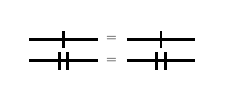
\begin{tikzpicture}[scale=0.62, every node/.style={font=\tiny, text=black}]
      \draw[black, line width=1.1pt, tk1] (0,0.22) -- (1.4,0.22);
      \draw[black, line width=1.1pt, tk1] (2.0,0.22) -- (3.4,0.22);
      \node at (1.7,0.22) {$=$};
      \draw[black, line width=1.1pt, tk2] (0,-0.22) -- (1.4,-0.22);
      \draw[black, line width=1.1pt, tk2] (2.0,-0.22) -- (3.4,-0.22);
      \node at (1.7,-0.22) {$=$};
    \end{tikzpicture}} \\ \hline

    \cnum{2} &
    \textbf{បូក/ដកអង្កត់រួម}\newline (\en{FJ+JG / RS+ST}) &
    ស្ពានរួមតភ្ជាប់អង្កត់ត្រង់ជួរ៖ $FG=FJ+JG=JG+GK=JK$ ឬ $RT=RS+ST=ST+TV=SV$ ។ &
    \raisebox{-0.35\height}{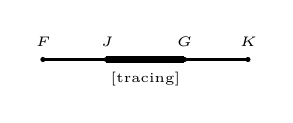
\begin{tikzpicture}[scale=0.62, every node/.style={font=\tiny, text=black}]
      \draw[black, line width=1.0pt] (0,0) -- (4.2,0);
      \draw[black, line width=2.2pt] (1.3,0) -- (2.9,0);
      \foreach \x/\l in {0/F, 1.3/J, 2.9/G, 4.2/K}{\fill[black] (\x,0) circle (1.5pt) node[above=1pt] {$\l$};}
      \node[below=1pt] at (2.1,0) {\en{[tracing]}};
    \end{tikzpicture}} \\ \hline

    \cnum{3} &
    \textbf{ជ្រុងរួម} (\en{Reflexive}) &
    អង្កត់ទ្រូងរួមក្នុងត្រីកោណជាប់គ្នា៖ $BC = CB$ ឬ $BD = BD$ (ប្រយ័ត្នលំដាប់កំពូលឆ្លាស់!) ។ &
    \raisebox{-0.35\height}{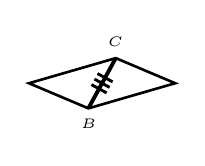
\begin{tikzpicture}[scale=0.58, every node/.style={font=\tiny, text=black}]
      \coordinate (A) at (0,0); \coordinate (B) at (1.3,-0.55); \coordinate (C) at (1.9,0.55); \coordinate (D) at (3.2,0);
      \draw[black, line width=0.95pt] (A)--(B)--(D)--(C)--cycle;
      \draw[black, line width=1.4pt, tk3] (B)--(C);
      \node[below=0.5pt] at (B) {$B$}; \node[above=0.5pt] at (C) {$C$};
    \end{tikzpicture}} \\ \hline

    \cnum{4} &
    \textbf{លក្ខខណ្ឌ ជ.ជ.ជ (\en{SSS})} &
    ជ្រុងទាំង ៣ ប៉ុនរៀងគ្នា $\Rightarrow \tri{ABC} \cg \tri{A'B'C'}$ ។ &
    \raisebox{-0.35\height}{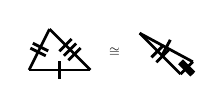
\begin{tikzpicture}[scale=0.52, every node/.style={font=\tiny, text=black}]
      \draw[black, line width=1.0pt, tk1] (0,0)--(1.5,0); \draw[black, line width=1.0pt, tk2] (0,0)--(0.5,1.0); \draw[black, line width=1.0pt, tk3] (1.5,0)--(0.5,1.0);
      \node at (2.1,0.45) {$\cg$};
      \draw[black, line width=1.0pt, tk1] (2.7,0.9)--(4.0,0.2); \draw[black, line width=1.0pt, tk2] (2.7,0.9)--(3.7,-0.1); \draw[black, line width=1.0pt, tk3] (4.0,0.2)--(3.7,-0.1);
    \end{tikzpicture}} \\ \hline

    \cnum{5} &
    \textbf{ធាតុត្រូវគ្នា} (មុំឈម) &
    មុំដែលឈមនឹងជ្រុងប៉ុនគ្នាមានរង្វាស់ស្មើគ្នា៖ $\ang{A}=\ang{A'}, \ang{B}=\ang{B'}, \ang{C}=\ang{C'}$ ។ &
    \raisebox{-0.35\height}{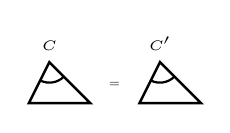
\begin{tikzpicture}[scale=0.52, every node/.style={font=\tiny, text=black}]
      \coordinate (u1) at (0,0); \coordinate (u2) at (1.5,0); \coordinate (u3) at (0.5,1.0);
      \draw[black, line width=0.9pt] (u1)--(u2)--(u3)--cycle;
      \pic[draw=black, line width=0.8pt, angle radius=2.6mm]{angle=u1--u3--u2};
      \node[above=0.5pt] at (u3) {$C$};
      \node at (2.1,0.45) {$=$};
      \coordinate (v1) at (2.7,0); \coordinate (v2) at (4.2,0); \coordinate (v3) at (3.2,1.0);
      \draw[black, line width=0.9pt] (v1)--(v2)--(v3)--cycle;
      \pic[draw=black, line width=0.8pt, angle radius=2.6mm]{angle=v1--v3--v2};
      \node[above=0.5pt] at (v3) {$C'$};
    \end{tikzpicture}} \\ \hline
  \end{tabular}

  \vspace{4pt}

  % --- ផ្នែកទី ៤៖ ប្រអប់ព្រមាន "ប្រយ័ត្នអន្ទាក់ ម.ម.ម (AAA)" vs "ជ.ជ.ជ (SSS)" ---
  \noindent
  \begin{minipage}[t]{8.75cm}
    \begin{tcolorbox}[
      enhanced, sharp corners, colback=white, colframe=black,
      boxrule=1.15pt, boxsep=1pt, equal height group=posterwarnSSS,
      top=3pt, bottom=3pt, left=5pt, right=5pt,
      title={\ding{51}\ \textbf{ត្រូវ៖ ករណី ជ.ជ.ជ (\en{SSS}) \en{--} រឹងថេរ ប៉ុនគ្នា!}},
      colbacktitle=headgray, coltitle=black, fonttitle=\fontsize{8.4pt}{11.5pt}\selectfont
    ]
      \centering
      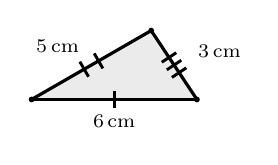
\begin{tikzpicture}[scale=0.70, every node/.style={font=\scriptsize, text=black}]
        \coordinate (A) at (0,0); \coordinate (B) at (3.0,0); \coordinate (C) at (2.17,1.25);
        \fill[panelgray] (A)--(B)--(C)--cycle;
        \draw[black, line width=1.15pt, tk1] (A)--(B) node[midway, below=1.5pt] {$6\unit{cm}$};
        \draw[black, line width=1.15pt, tk2] (A)--(C) node[midway, above left=0.5pt] {$5\unit{cm}$};
        \draw[black, line width=1.15pt, tk3] (B)--(C) node[pos=0.35, above right=2.5pt] {$3\unit{cm}$};
        \fill[black] (A) circle (1.5pt) (B) circle (1.5pt) (C) circle (1.5pt);
      \end{tikzpicture}
      \par\vspace{1.5pt}\fontsize{7.9pt}{11.2pt}\selectfont
      ជ្រុងទាំង ៣ ($6, 5, 3\unit{cm}$) \textbf{ចាក់សោមុំទាំង ៣ ដោយស្វ័យប្រវត្តិ} $\Rightarrow$ បង្កើតត្រីកោណ\textbf{តែមួយគត់} ($\tri{ABC}\cg\tri{A'B'C'}$)!
    \end{tcolorbox}
  \end{minipage}\hfill
  \begin{minipage}[t]{8.75cm}
    \begin{tcolorbox}[
      enhanced, sharp corners, colback=white, colframe=black,
      boxrule=1.15pt, boxsep=1pt, equal height group=posterwarnSSS,
      top=3pt, bottom=3pt, left=5pt, right=5pt,
      title={\ding{55}\ \textbf{ប្រយ័ត្នអន្ទាក់ ម.ម.ម (\en{AAA}) \en{--} មិនប៉ុនគ្នាទេ!}},
      colbacktitle=midgray, coltitle=black, fonttitle=\fontsize{8.4pt}{11.5pt}\selectfont
    ]
      \centering
      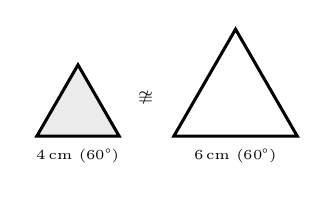
\begin{tikzpicture}[scale=0.58, every node/.style={font=\scriptsize, text=black}]
        \fill[panelgray] (0,0) -- (1.8,0) -- (0.9,1.56) -- cycle;
        \draw[black, line width=1.1pt] (0,0) -- (1.8,0) -- (0.9,1.56) -- cycle;
        \node[below=1pt, font=\tiny] at (0.9,0) {$4\unit{cm}$ ($60^\circ$)};
        \node[font=\scriptsize] at (2.4, 0.85) {$\ncg$};
        \fill[white] (3.0,0) -- (5.7,0) -- (4.35,2.34) -- cycle;
        \draw[black, line width=1.1pt] (3.0,0) -- (5.7,0) -- (4.35,2.34) -- cycle;
        \node[below=1pt, font=\tiny] at (4.35,0) {$6\unit{cm}$ ($60^\circ$)};
      \end{tikzpicture}
      \par\vspace{1.5pt}\fontsize{7.9pt}{11.2pt}\selectfont
      មុំ ៣ ស្មើគ្នា ($60^\circ\text{-}60^\circ\text{-}60^\circ$) គ្រាន់តែ\textbf{ពង្រីក/បង្រួមទំហំ} មិនធានាជ្រុងស្មើទេ ($\tri{PQR}\ncg\tri{P'Q'R'}$)!
    \end{tcolorbox}
  \end{minipage}
\end{tcolorbox}

\clearpage

% ============================================================================
% ទំព័រទី ៥៖ កាតវិនិច្ឆ័យរហ័ស ៦០–៩០ វិនាទី "កាត A–D" & តារាងចម្លើយគ្រូ — E5 Evaluate
% ============================================================================
\pagebanner{សម្ភារៈទី ៥៖ កាតវិនិច្ឆ័យរហ័ស «កាត \enbf{A--D}» \enbf{(60--90} វិនាទី\enbf{) \&} ចម្លើយគ្រូ}{ទំព័រ ៥/៦ \en{-- E5 Evaluate}}

{\fontsize{8.5pt}{12pt}\selectfont
\textbf{វិធីលេងក្នុងថ្នាក់៖} គ្រូលើកកាតម្ដងមួយ $\rightarrow$ សិស្សផ្ទៀង ៣ ជ្រុង/កំពូលឈម $\rightarrow$ លើក \textbf{មេដៃឡើង (ពិត \ding{51})} ឬ \textbf{ខ្វែងដៃ (ខុស/អន្ទាក់ \ding{55})} + បង្ហាញម្រាម \en{1--3}។}

\vspace{4pt}

% --- ជួរទី ១៖ កាត A & កាត B ---
\noindent
\begin{tcolorbox}[
  enhanced, sharp corners, colback=white, colframe=white,
  borderline={1.0pt}{0pt}{black, dashed},
  width=9.25cm, equal height group=sssfoilrow1, nobeforeafter,
  boxsep=1pt, top=5pt, bottom=5pt, left=6pt, right=6pt
]
  \noindent\colorbox{black}{\textcolor{white}{\Large\textbf{\en{ A }}}}\hspace{0.25cm}{\fontsize{9.3pt}{12.5pt}\selectfont\textbf{កាត \en{A} ៖ ជ.ជ.ជ បង្វិល\en{--}ឆ្លុះ $\approx 135^\circ$}}\par\vspace{2pt}
  \begin{center}
  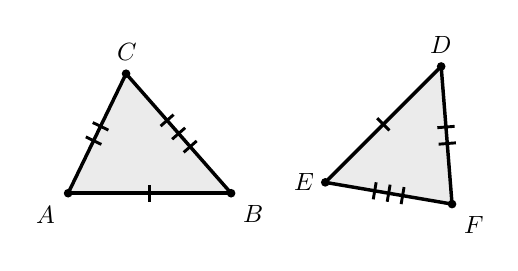
\begin{tikzpicture}[scale=0.92, every node/.style={font=\small, text=black}]
    \coordinate (A) at (0,0); \coordinate (B) at (2.25,0); \coordinate (C) at (0.80,1.65);
    \fill[panelgray] (A)--(B)--(C)--cycle;
    \draw[black, line width=1.25pt, tk1] (A)--(B);
    \draw[black, line width=1.25pt, tk2] (A)--(C);
    \draw[black, line width=1.25pt, tk3] (B)--(C);
    \fill[black] (A) circle (1.7pt) (B) circle (1.7pt) (C) circle (1.7pt);
    \node[below left=1pt] at (A) {$A$}; \node[below right=1pt] at (B) {$B$}; \node[above=1pt] at (C) {$C$};
    % បង្វិល-ឆ្លុះ ~135°
    \coordinate (D) at (5.15, 1.75); \coordinate (E) at (3.55, 0.15); \coordinate (F) at (5.30, -0.15);
    \fill[panelgray] (D)--(E)--(F)--cycle;
    \draw[black, line width=1.25pt, tk1] (D)--(E);
    \draw[black, line width=1.25pt, tk2] (D)--(F);
    \draw[black, line width=1.25pt, tk3] (E)--(F);
    \fill[black] (D) circle (1.7pt) (E) circle (1.7pt) (F) circle (1.7pt);
    \node[above=1pt] at (D) {$D$}; \node[left=1pt] at (E) {$E$}; \node[below right=1pt] at (F) {$F$};
  \end{tikzpicture}
  \end{center}
  \vfill
  \begin{tcolorbox}[enhanced, sharp corners, colback=panelgray, colframe=black, boxrule=0.8pt, boxsep=1pt, top=4pt, bottom=4pt, left=5pt, right=5pt]
    \centering\fontsize{9.0pt}{12.5pt}\selectfont
    \textbf{សំណួរ៖} តើ $\tri{ABC} \cg \tri{DEF}$ តាម \textbf{ជ.ជ.ជ} ឬទេ?\\[2pt]
    \chkbox\ មេដៃឡើង (\ding{51} ពិត) \hspace{0.4cm} \chkbox\ ខ្វែងដៃ (\ding{55} ខុស)
  \end{tcolorbox}
\end{tcolorbox}%
\hfill
\begin{tcolorbox}[
  enhanced, sharp corners, colback=white, colframe=white,
  borderline={1.0pt}{0pt}{black, dashed},
  width=9.25cm, equal height group=sssfoilrow1, nobeforeafter,
  boxsep=1pt, top=5pt, bottom=5pt, left=6pt, right=6pt
]
  \noindent\colorbox{black}{\textcolor{white}{\Large\textbf{\en{ B }}}}\hspace{0.25cm}{\fontsize{9.3pt}{12.5pt}\selectfont\textbf{កាត \en{B} ៖ អន្ទាក់ ម.ម.ម (\en{AAA} $60^\circ$) $4\unit{cm}$ vs $6\unit{cm}$}}\par\vspace{2pt}
  \begin{center}
  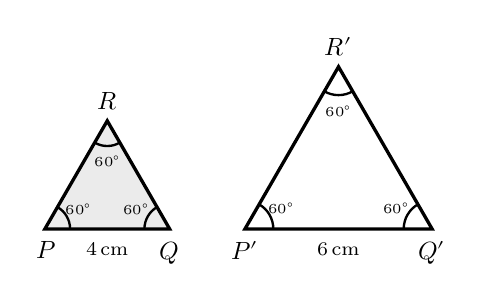
\begin{tikzpicture}[scale=0.66, every node/.style={font=\small, text=black}]
    % 4 cm
    \coordinate (P) at (0,0); \coordinate (Q) at (2.4,0); \coordinate (R) at (1.2, 2.08);
    \fill[panelgray] (P)--(Q)--(R)--cycle;
    \draw[black, line width=1.2pt] (P)--(Q)--(R)--cycle;
    \pic[draw=black, line width=0.85pt, angle radius=3.2mm]{angle=Q--P--R};
    \pic[draw=black, line width=0.85pt, angle radius=3.2mm]{angle=R--Q--P};
    \pic[draw=black, line width=0.85pt, angle radius=3.2mm]{angle=P--R--Q};
    \node[font=\tiny] at ($(P)+(30:0.75)$) {$60^\circ$};
    \node[font=\tiny] at ($(Q)+(150:0.75)$) {$60^\circ$};
    \node[font=\tiny] at ($(R)+(-90:0.78)$) {$60^\circ$};
    \node[below=1.5pt, font=\scriptsize] at (1.2,0) {$4\unit{cm}$};
    \node[below=1pt] at (P) {$P$}; \node[below=1pt] at (Q) {$Q$}; \node[above=0.5pt] at (R) {$R$};
    % 6 cm (shifted right to 3.85 so Q and P' never touch!)
    \coordinate (Pp) at (3.85,0); \coordinate (Qp) at (7.45,0); \coordinate (Rp) at (5.65, 3.12);
    \fill[white] (Pp)--(Qp)--(Rp)--cycle;
    \draw[black, line width=1.2pt] (Pp)--(Qp)--(Rp)--cycle;
    \pic[draw=black, line width=0.85pt, angle radius=3.6mm]{angle=Qp--Pp--Rp};
    \pic[draw=black, line width=0.85pt, angle radius=3.6mm]{angle=Rp--Qp--Pp};
    \pic[draw=black, line width=0.85pt, angle radius=3.6mm]{angle=Pp--Rp--Qp};
    \node[font=\tiny] at ($(Pp)+(30:0.80)$) {$60^\circ$};
    \node[font=\tiny] at ($(Qp)+(150:0.80)$) {$60^\circ$};
    \node[font=\tiny] at ($(Rp)+(-90:0.85)$) {$60^\circ$};
    \node[below=1.5pt, font=\scriptsize] at (5.65,0) {$6\unit{cm}$};
    \node[below=1pt] at (Pp) {$P'$}; \node[below=1pt] at (Qp) {$Q'$}; \node[above=0.5pt] at (Rp) {$R'$};
  \end{tikzpicture}
  \end{center}
  \vfill
  \begin{tcolorbox}[enhanced, sharp corners, colback=panelgray, colframe=black, boxrule=0.8pt, boxsep=1pt, top=4pt, bottom=4pt, left=5pt, right=5pt]
    \centering\fontsize{9.0pt}{12.5pt}\selectfont
    \textbf{សំណួរ៖} មុំ ៣ ស្មើគ្នា ($60^\circ$) តើ $\tri{PQR} \cg \tri{P'Q'R'}$ ឬទេ?\\[2pt]
    \chkbox\ មេដៃឡើង (\ding{51} ពិត) \hspace{0.4cm} \chkbox\ ខ្វែងដៃ (\ding{55} ខុស)
  \end{tcolorbox}
\end{tcolorbox}

\vspace{6pt}

% --- ជួរទី ២៖ កាត C & កាត D ---
\noindent
\begin{tcolorbox}[
  enhanced, sharp corners, colback=white, colframe=white,
  borderline={1.0pt}{0pt}{black, dashed},
  width=9.25cm, equal height group=sssfoilrow2, nobeforeafter,
  boxsep=1pt, top=5pt, bottom=5pt, left=6pt, right=6pt
]
  \noindent\colorbox{black}{\textcolor{white}{\Large\textbf{\en{ C }}}}\hspace{0.25cm}{\fontsize{9.3pt}{12.5pt}\selectfont\textbf{កាត \en{C} ៖ អន្ទាក់កំណាត់អង្កត់ $FJ=GK$ (គ្មានស្ពាន)}}\par\vspace{2pt}
  \begin{center}
  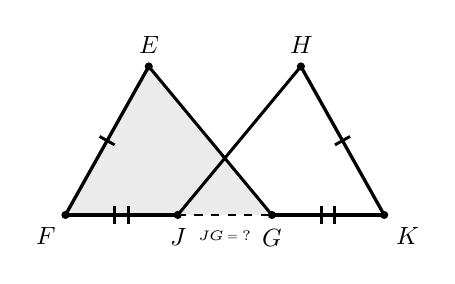
\begin{tikzpicture}[scale=0.92, every node/.style={font=\small, text=black}]
    \coordinate (F) at (0,0); \coordinate (J) at (1.55,0); \coordinate (G) at (2.85,0); \coordinate (K) at (4.40,0);
    \coordinate (E) at (1.15, 2.05); \coordinate (H) at (3.25, 2.05);
    \fill[panelgray] (E)--(F)--(G)--cycle;
    \draw[black, line width=1.1pt] (E)--(G) (H)--(J);
    \draw[black, line width=1.2pt, tk1] (E)--(F);
    \draw[black, line width=1.2pt, tk1] (H)--(K);
    \draw[black, line width=1.2pt, tk2] (F)--(J);
    \draw[black, line width=1.2pt, tk2] (G)--(K);
    \draw[black, line width=1.0pt, dashed] (J)--(G);
    \node[below=2pt, font=\tiny] at (2.20, 0) {$JG = ?$};
    \fill[black] (F) circle (1.6pt) node[below left=1pt] {$F$};
    \fill[black] (J) circle (1.6pt) node[below=1.5pt] {$J$};
    \fill[black] (G) circle (1.6pt) node[below=1.5pt] {$G$};
    \fill[black] (K) circle (1.6pt) node[below right=1pt] {$K$};
    \fill[black] (E) circle (1.6pt) node[above=1pt] {$E$};
    \fill[black] (H) circle (1.6pt) node[above=1pt] {$H$};
  \end{tikzpicture}
  \end{center}
  {\centering\fontsize{8.0pt}{11pt}\selectfont គេអះអាង៖ «មាន $EF=HK$, $FJ=GK$, គ្រប់គ្រាន់តាម ជ.ជ.ជ!»\par}
  \vfill
  \begin{tcolorbox}[enhanced, sharp corners, colback=panelgray, colframe=black, boxrule=0.8pt, boxsep=1pt, top=4pt, bottom=4pt, left=5pt, right=5pt]
    \centering\fontsize{9.0pt}{12.5pt}\selectfont
    \textbf{សំណួរ៖} សរសេរថា $\tri{EFG}\cg\tri{HKJ}$ ភ្លាម ត្រូវឬខុស?\\[2pt]
    \chkbox\ មេដៃឡើង (\ding{51} ពិត) \hspace{0.4cm} \chkbox\ ខ្វែងដៃ (\ding{55} ខុស)
  \end{tcolorbox}
\end{tcolorbox}%
\hfill
\begin{tcolorbox}[
  enhanced, sharp corners, colback=white, colframe=white,
  borderline={1.0pt}{0pt}{black, dashed},
  width=9.25cm, equal height group=sssfoilrow2, nobeforeafter,
  boxsep=1pt, top=5pt, bottom=5pt, left=6pt, right=6pt
]
  \noindent\colorbox{black}{\textcolor{white}{\Large\textbf{\en{ D }}}}\hspace{0.25cm}{\fontsize{9.3pt}{12.5pt}\selectfont\textbf{កាត \en{D} ៖ អន្ទាក់លំដាប់កំពូលខុស $\tri{ABC}\cg\tri{BDC}$}}\par\vspace{2pt}
  \begin{center}
  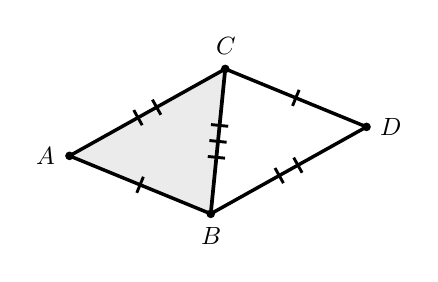
\begin{tikzpicture}[scale=0.92, every node/.style={font=\small, text=black}]
    % ចតុកោណ ABDC (រចនាប័ទ្មលំហាត់ ៩ ទំព័រ ១៦៥)
    \coordinate (A) at (0, 0.35);
    \coordinate (B) at (1.95, -0.45);
    \coordinate (C) at (2.15, 1.55);
    \coordinate (D) at (4.10, 0.75);
    \fill[panelgray] (A)--(B)--(C)--cycle;
    \draw[black, line width=1.25pt, tk1] (A)--(B);
    \draw[black, line width=1.25pt, tk1] (C)--(D);
    \draw[black, line width=1.25pt, tk2] (A)--(C);
    \draw[black, line width=1.25pt, tk2] (B)--(D);
    \draw[black, line width=1.35pt, tk3] (B)--(C);
    \fill[black] (A) circle (1.7pt) node[left=1.5pt] {$A$};
    \fill[black] (B) circle (1.7pt) node[below=1.5pt] {$B$};
    \fill[black] (C) circle (1.7pt) node[above=1.5pt] {$C$};
    \fill[black] (D) circle (1.7pt) node[right=1.5pt] {$D$};
  \end{tikzpicture}
  \end{center}
  {\centering\fontsize{8.0pt}{11pt}\selectfont $AB=CD$, $AC=BD$, $BC$ រួម ។ សិស្សសរសេរ $\tri{ABC}\cg\tri{BDC}$ ។\par}
  \vfill
  \begin{tcolorbox}[enhanced, sharp corners, colback=panelgray, colframe=black, boxrule=0.8pt, boxsep=1pt, top=4pt, bottom=4pt, left=5pt, right=5pt]
    \centering\fontsize{9.0pt}{12.5pt}\selectfont
    \textbf{សំណួរ៖} តើការសរសេរ $\tri{ABC} \cg \tri{BDC}$ ត្រឹមត្រូវឬខុស?\\[2pt]
    \chkbox\ មេដៃឡើង (\ding{51} ពិត) \hspace{0.4cm} \chkbox\ ខ្វែងដៃ (\ding{55} ខុស)
  \end{tcolorbox}
\end{tcolorbox}

\vspace{6pt}

% --- ខ្សែកាត់ & បន្ទះចម្លើយសម្រាប់គ្រូ ---
\noindent\scissors\ \dotfill\ \textbf{កាត់ទុកសម្រាប់គ្រូ (\en{Teacher Mini Answer \& Remediation Key})} \dotfill\ \scissors

\vspace{4pt}
\begin{tcolorbox}[
  enhanced, sharp corners, colback=panelgray, colframe=black,
  boxrule=1.0pt, boxsep=1pt, top=4pt, bottom=4pt, left=5pt, right=5pt
]
  \fontsize{7.8pt}{11.0pt}\selectfont
  \renewcommand{\arraystretch}{1.10}
  \begin{tabular}{|L{4.0cm}|L{4.2cm}|L{4.3cm}|L{4.5cm}|}
    \hline
    \cellcolor{headgray}\textbf{កាត \en{A} ៖ មេដៃឡើង (\ding{51})} &
    \cellcolor{headgray}\textbf{កាត \en{B} ៖ ខ្វែងដៃ (\ding{55})} &
    \cellcolor{headgray}\textbf{កាត \en{C} ៖ ខ្វែងដៃ (\ding{55})} &
    \cellcolor{headgray}\textbf{កាត \en{D} ៖ ខ្វែងដៃ (\ding{55})} \\ \hline
    $\tri{ABC}\cg\tri{DEF}$ តាម \textbf{ជ.ជ.ជ} ទោះបង្វិល\en{--}ឆ្លុះ $\approx 135^\circ$។ ផ្ទៀងសញ្ញា \tickone, \ticktwo, \tickthree\ និងកំពូលឈមជ្រុង! &
    \textbf{អន្ទាក់ ម.ម.ម (\en{AAA})}! មុំ $60^\circ$ ស្មើគ្នាគ្រាន់តែរូបដូចគ្នា តែជ្រុង $4\unit{cm} \neq 6\unit{cm}$ ($\ncg$)។ &
    \textbf{ខ្វះស្ពាន $JG$ \& ជ្រុងទី ៣!} $FJ$ មិនមែនជ្រុង $\tri{EFG}$ ទេ; ត្រូវរក $EG=HJ$ និងបូក $FG=FJ+JG=JK$ (\cnum{2})។ &
    \textbf{ខុសលំដាប់កំពូល!} ឈម $AC$ (\ticktwo) គឺ $B$ ទល់ឈម $BD$ (\ticktwo) គឺ $C$ $\Rightarrow$ ត្រូវសរសេរ $\tri{ABC}\cg\tri{DCB}$! \\ \hline
  \end{tabular}
  \par\vspace{2.5pt}
  \textbf{ត្រួតទំនុកចិត្ត (ម្រាម ១\en{--}៣)៖} ១ ម្រាម = ហៅដៃគូចង្អុលជ្រុងឈមកំពូលឡើងវិញ \hspace{0.25cm}\en{|}\hspace{0.25cm} ២ ម្រាម = ផ្ទៀងធនាគារ \cnum{1}--\cnum{5} \hspace{0.25cm}\en{|}\hspace{0.25cm} ៣ ម្រាម = ច្បាស់ ១០០\%
\end{tcolorbox}

\clearpage

% ============================================================================
% ទំព័រទី ៦៖ ប័ណ្ណកិច្ចការផ្ទះ ជំហានទី ៥ — ៤ ប័ណ្ណក្នុង ១ ទំព័រ A4 (4-up: HW #4 & #9)
% ============================================================================
\pagebanner{សម្ភារៈទី ៦៖ ប័ណ្ណកិច្ចការផ្ទះ ជំហានទី ៥ \enbf{--} ៤ ប័ណ្ណក្នុង ១ ទំព័រ \enbf{A4}}{ទំព័រ ៦/៦ \en{--} ជំហានទី ៥ (កាត់ ៤ ប័ណ្ណ \scissors)}

% ម៉ាក្រូប័ណ្ណកិច្ចការផ្ទះ ៤-up (ផ្ទៀង ១០០% នឹងលំហាត់ទី ៤ ទំព័រ ១៦៤ និងលំហាត់ទី ៩ ទំព័រ ១៦៥)
\newcommand{\hwslipFour}[1]{%
\begin{tcolorbox}[
  enhanced, sharp corners, colback=white, colframe=white,
  borderline={0.95pt}{0pt}{black, dashed},
  width=9.25cm, equal height group=hwquad, nobeforeafter,
  boxsep=1pt, top=3.5pt, bottom=3.5pt, left=4.5pt, right=4.5pt
]
  \begin{tcolorbox}[
    enhanced, sharp corners, colback=headgray, colframe=black,
    boxrule=0.7pt, boxsep=1pt, top=2pt, bottom=2pt, left=4pt, right=4pt, after skip=4pt
  ]
    \fontsize{7.6pt}{10.5pt}\selectfont
    \textbf{\scissors\ កិច្ចការផ្ទះ (#1) \en{|} ១.២.៣ ជ.ជ.ជ} \hfill \textbf{សុក្រ ២៧/១១/២៦}\\[1.5pt]
    ឈ្មោះ៖ $\underline{\hspace{4.0cm}}$ \hspace{0.2cm} ថ្នាក់៖ $\underline{\hspace{1.0cm}}$
  \end{tcolorbox}

  % --- លំហាត់ទី ៤ (សៀវភៅទំព័រ ១៦៤) ---
  \noindent
  \begin{minipage}[c]{5.15cm}
    \fontsize{7.6pt}{11.0pt}\selectfont
    \textbf{លំហាត់ទី ៤ (ទំព័រ ១៦៤)៖} គេឱ្យ $AB = BC$ និង $AD = CD$~។ ប្រៀបធៀប $\tri{AED}$ និង $\tri{CED}$~។\\
    {\fontsize{6.9pt}{9.8pt}\selectfont\textit{តម្រុយ៖} $\tri{ABD}\cg\tri{CBD}$ (\cnum{4} ជ.ជ.ជ) $\Rightarrow \ang{ADE}=\ang{CDE}$ (\cnum{5}) $\Rightarrow$ ជ.ម.ជ!}
  \end{minipage}\hfill
  \begin{minipage}[c]{3.25cm}
    \centering
    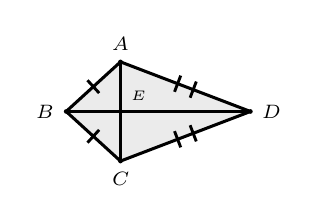
\begin{tikzpicture}[scale=0.60, every node/.style={font=\scriptsize, text=black}]
      % Kite ABCD (Book p. 164 #4)
      \coordinate (B) at (-1.15, 0);
      \coordinate (A) at (0, 1.05);
      \coordinate (C) at (0, -1.05);
      \coordinate (D) at (2.75, 0);
      \coordinate (E) at (0, 0);
      \fill[panelgray] (A)--(B)--(C)--(D)--cycle;
      \draw[black, line width=1.1pt, tk1] (A)--(B);
      \draw[black, line width=1.1pt, tk1] (B)--(C);
      \draw[black, line width=1.1pt, tk2] (A)--(D);
      \draw[black, line width=1.1pt, tk2] (C)--(D);
      \draw[black, line width=0.95pt] (A)--(C) (B)--(D);
      \fill[black] (A) circle (1.4pt) node[above=0.5pt] {$A$};
      \fill[black] (B) circle (1.4pt) node[left=1pt] {$B$};
      \fill[black] (C) circle (1.4pt) node[below=0.5pt] {$C$};
      \fill[black] (D) circle (1.4pt) node[right=1pt] {$D$};
      \fill[black] (E) circle (1.4pt) node[above right=0.5pt, font=\tiny] {$E$};
    \end{tikzpicture}
  \end{minipage}

  \vspace{4pt}
  \hrule height 0.5pt
  \vspace{4pt}

  % --- លំហាត់ទី ៩ (សៀវភៅទំព័រ ១៦៥) ---
  \noindent
  \begin{minipage}[c]{5.15cm}
    \fontsize{7.6pt}{11.0pt}\selectfont
    \textbf{លំហាត់ទី ៩ (ទំព័រ ១៦៥)៖} គេឱ្យ $AB = CD$ និង $AC = BD$ ដូចរូប~។ ប្រៀបធៀប $\tri{ABC}$ និង $\tri{BDC}$~។\\
    {\fontsize{6.9pt}{9.8pt}\selectfont\textit{ប្រយ័ត្នលំដាប់កំពូល៖} $BC=CB$ (\cnum{3}) $\Rightarrow \tri{ABC}\cg\tri{\underline{\hspace{0.65cm}}}$!}
  \end{minipage}\hfill
  \begin{minipage}[c]{3.25cm}
    \centering
    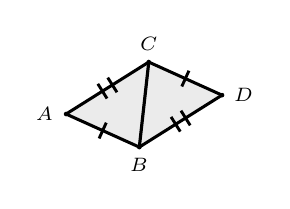
\begin{tikzpicture}[scale=0.60, every node/.style={font=\scriptsize, text=black}]
      % Quad ABDC (Book p. 165 #9)
      \coordinate (A) at (0, 0.25);
      \coordinate (B) at (1.55, -0.45);
      \coordinate (C) at (1.75, 1.35);
      \coordinate (D) at (3.30, 0.65);
      \fill[panelgray] (A)--(B)--(D)--(C)--cycle;
      \draw[black, line width=1.1pt, tk1] (A)--(B);
      \draw[black, line width=1.1pt, tk1] (C)--(D);
      \draw[black, line width=1.1pt, tk2] (A)--(C);
      \draw[black, line width=1.1pt, tk2] (B)--(D);
      \draw[black, line width=1.15pt] (B)--(C);
      \fill[black] (A) circle (1.4pt) node[left=1pt] {$A$};
      \fill[black] (B) circle (1.4pt) node[below=0.5pt] {$B$};
      \fill[black] (C) circle (1.4pt) node[above=0.5pt] {$C$};
      \fill[black] (D) circle (1.4pt) node[right=1pt] {$D$};
    \end{tikzpicture}
  \end{minipage}

  \vspace{4pt}
  \begin{tcolorbox}[
    enhanced, sharp corners, colback=panelgray, colframe=black,
    boxrule=0.75pt, boxsep=1pt, top=3pt, bottom=3pt, left=4pt, right=4pt
  ]
    \fontsize{7.15pt}{10.3pt}\selectfont
    \textbf{ផ្ទៀងខ្លួនឯង (\en{Warrant \cnum{1}--\cnum{5}})៖}
    \chkbox\ គូស \tickone, \ticktwo, \tickthree\ លើរូប (រួមទាំង \cnum{3} $BD=BD, BC=CB$)~។\\
    \chkbox\ ដាក់លេខ \cnum{1}--\cnum{5} គ្រប់បន្ទាត់ (លំ.៤៖ \cnum{1},\cnum{3},\cnum{4},\cnum{5}; លំ.៩៖ \cnum{1},\cnum{3},\cnum{4})~។\\
    \chkbox\ ផ្ទៀងកំពូលឈមជ្រុងស្មើ (លំ.៩៖ $A\leftrightarrow D, B\leftrightarrow C, C\leftrightarrow B$) \& $=$ ទល់ $\cg$~។
  \end{tcolorbox}
\end{tcolorbox}%
}

\noindent
\hwslipFour{ប័ណ្ណទី ១}\hfill\hwslipFour{ប័ណ្ណទី ២}

\vspace{8pt}
\noindent\scissors\ \dotfill\ \textbf{កាត់តាមស្នាមចុចចែកជា ៤ ប័ណ្ណ (\en{Cut Along Dashed Lines})} \dotfill\ \scissors
\vspace{8pt}

\noindent
\hwslipFour{ប័ណ្ណទី ៣}\hfill\hwslipFour{ប័ណ្ណទី ៤}

\end{document}
